\chapter{\label{ch:3-anomalies}The LSND and MiniBooNE anomalies}

\minitoc

The LSND experiment observed an excess of $\bar{\nu}_{e}$ in a primarily $\bar{\nu}_{\mu}$ beam in 2001. The MiniBooNE experiment, built to confirm or rule out the anomaly, observed a significant excess of $\nu_{e}$-like ($\bar{\nu}_{e}$-like) events in a primarily $\nu_{\mu}$ ($\bar{\nu}_{\mu}$) beam. Several other neutrino experiments have shown results not fully compatible with the three-flavour scenario and they will be briefly described.  A summary of the global picture of the short-baseline anomalies will also be provided.

\section{The LSND experiment}
The Liquid Scintillator Neutrino Detector (LSND) was an experiment at the Los Alamos National Laboratory which aimed to detect $\bar{\nu}_e$ interactions in a mainly $\bar{\nu}_{\mu}$ beam. The neutrino beam was produced by firing an 800 MeV proton beam into a target, producing charged pions, which were stopped in a beam dump. The $\pi^-$ part was electromagnetically captured by the nucleus, while the $\pi^+$ component initiated the decay chain:
\begin{align}
    \pi^+ \rightarrow & \mu^+\nu_{\mu}\\
    & \rotatebox[origin=c]{180}{$\Lsh$}	 \mu^{+} \rightarrow e^+\bar{\nu}_{\mu}\nu_{e}.
\end{align}
Kinematically, it is possible to distinguish between the neutrino beam produced by decays at rest (DAR), and the neutrino beam produced by decays in flight (DIF). In LSND, this was achieved by looking at events with energies above (below) 60~MeV to select the DIF (DAR) beam, since the maximum energy for a $\bar{\nu}_{\mu}$ produced by a stopping muon is 52.8~MeV ($m_{\mu}/2$) .

The detector was filled with 167~t of mineral oil (CH$_2$) and doped with 0.031~g/l of organic scintillation material (butyl-PBD).

\begin{figure}[htbp]
    \centering
    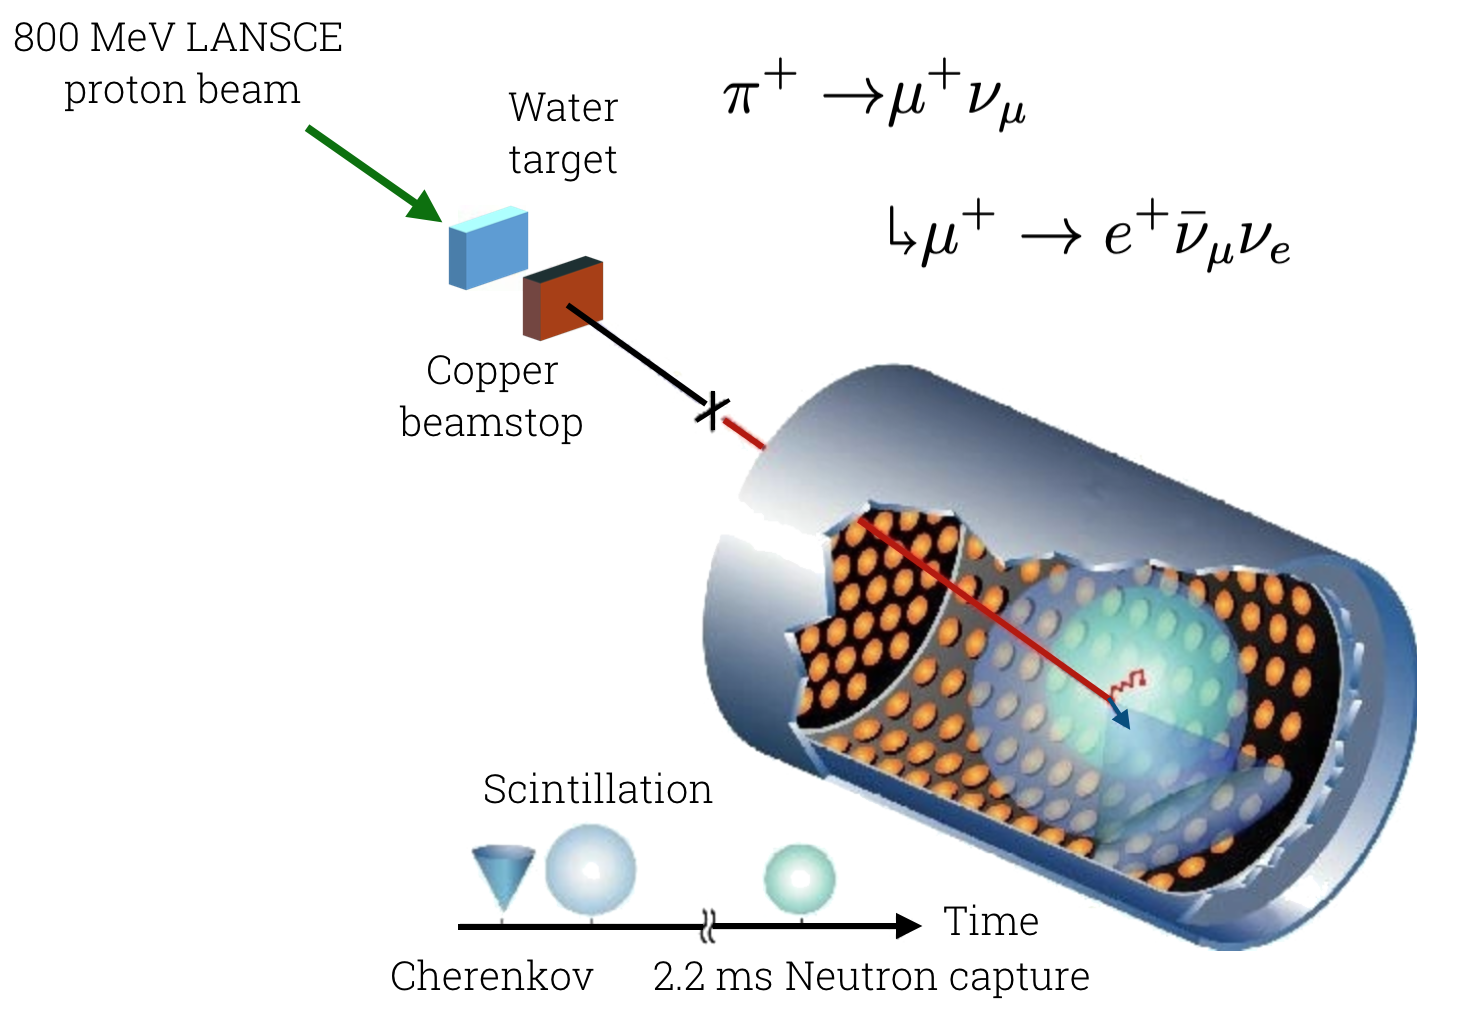
\includegraphics[width=0.9\linewidth]{figures/lsnd_exp.png}
    \caption{A schematic of the LSND experiment and its detection technique: the inverse $\beta$-decay of the neutrinos in the detector produce Cherenkov and scintillation light, in delayed coincidence with the light emitted by the neutron capture.}
    \label{fig:lsnd_exp}
\end{figure}

The $\bar{\nu}_e$ interactions were detected via an inverse $\beta$-decay process and tagged with a delayed coincidence between the positron and the subsequent neutron capture, in a fashion similar to the Cowan and Reines experiment. A schematic of the LSND experiment and its detection technique is shown in Figure \ref{fig:lsnd_exp}.

LSND found an excess of $\bar{\nu}_e$ interactions in the DAR $\bar{\nu}_{\mu}$ beam with a significance of $3.8\sigma$, which could be explained as $\bar{\nu}_\mu$ oscillating into $\bar{\nu}_e$ (Figure \ref{fig:resultlsnd}). Given the $L/E\approx0.75$~m/MeV of the experiment, the mass splitting term obtained with LSND data is $\Delta m_{\mathrm{LSND}}^2\approx1$~eV. This value is one order of magnitude larger than the mass splitting terms obtained with any other reactor, accelerator, atmospheric, or solar experiment \cite{Aguilar:2001ty}. An excess of $\nu_{e}$ was found also in the DIF $\nu_{\mu}$ beam, compatible with the $\bar{\nu}_\mu \rightarrow \bar{\nu}_e$ oscillation result \cite{Athanassopoulos:1997pv}. 

\begin{figure}[htbp]
  \begin{subfigure}{0.48\textwidth}
    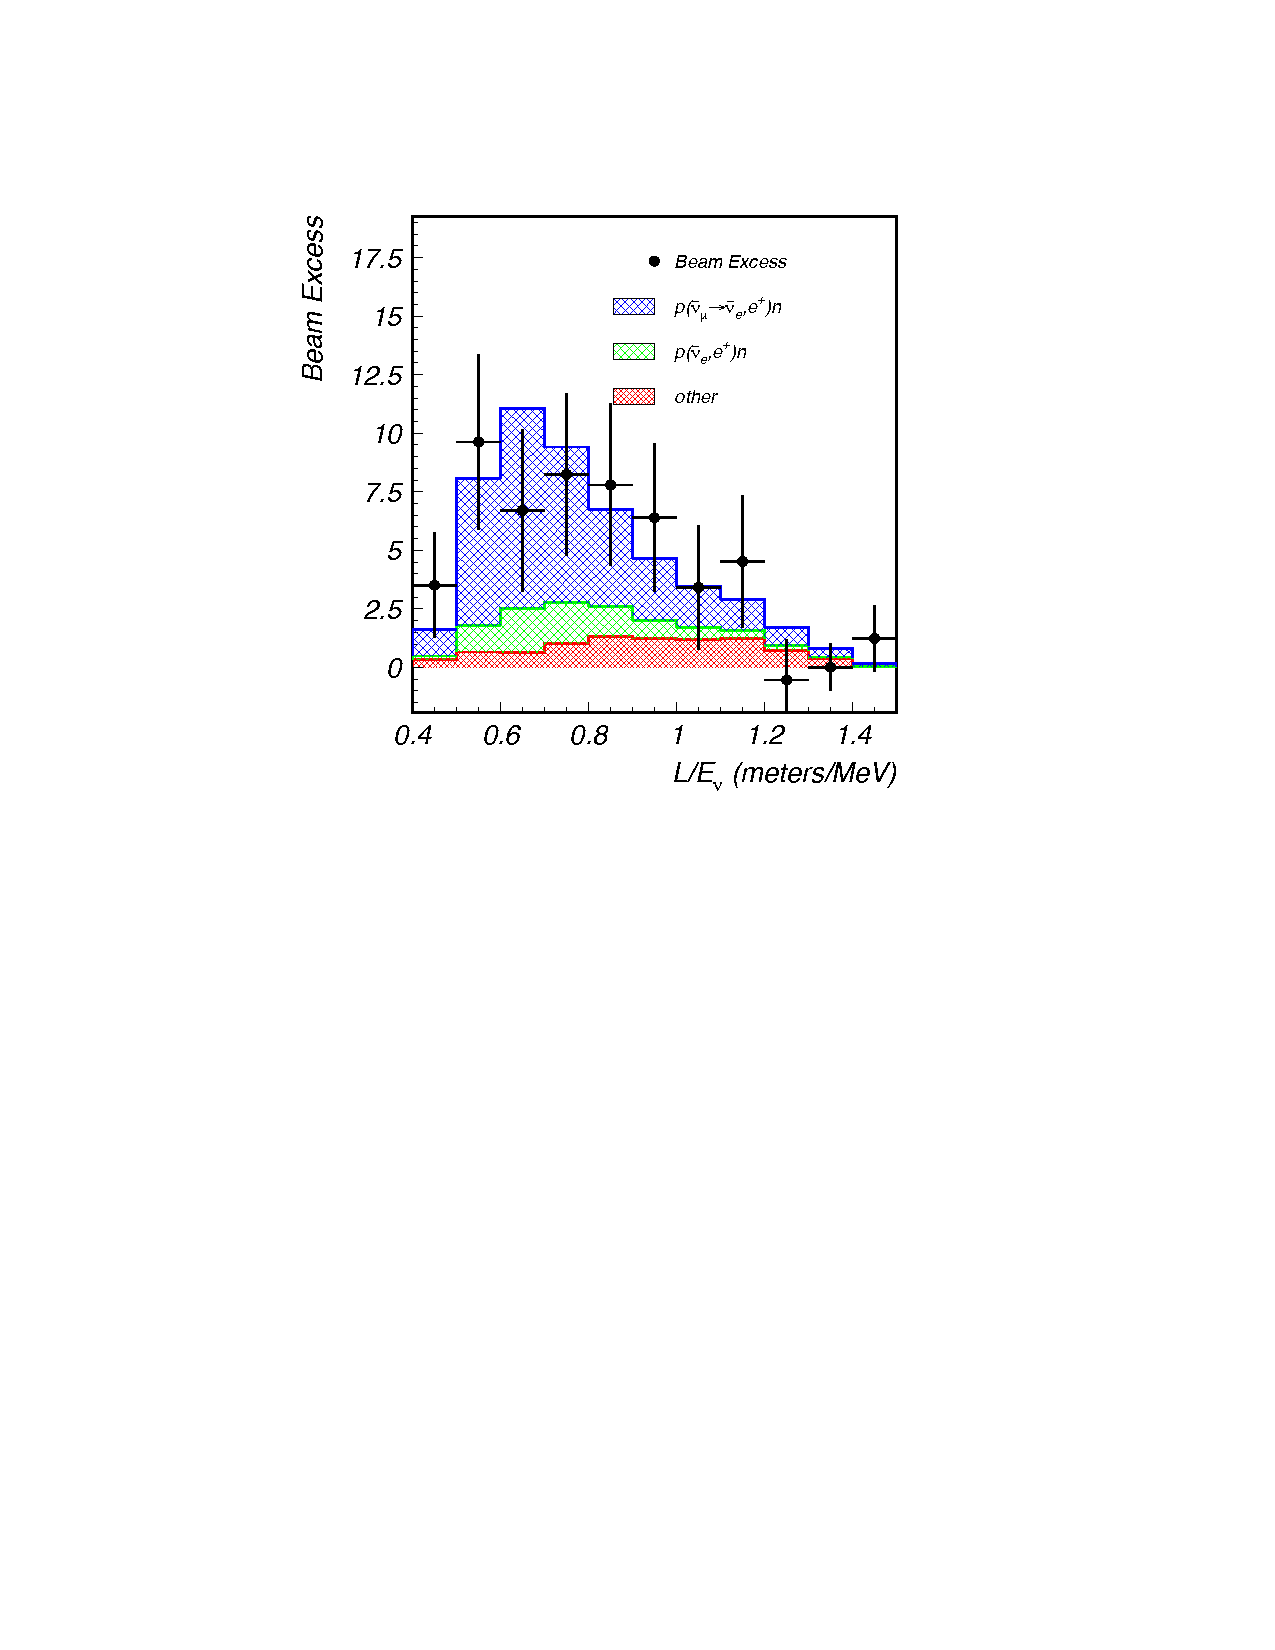
\includegraphics[height=\linewidth]{figures/lsndresult.pdf}
    \caption{$L/E_{\nu}$ distribution for the $\bar{\nu}_{e}$ events in the LSND experiment.}\label{fig:resultlsnd}
  \end{subfigure}\hfill
  \begin{subfigure}{0.48\textwidth}
    \begin{center}
        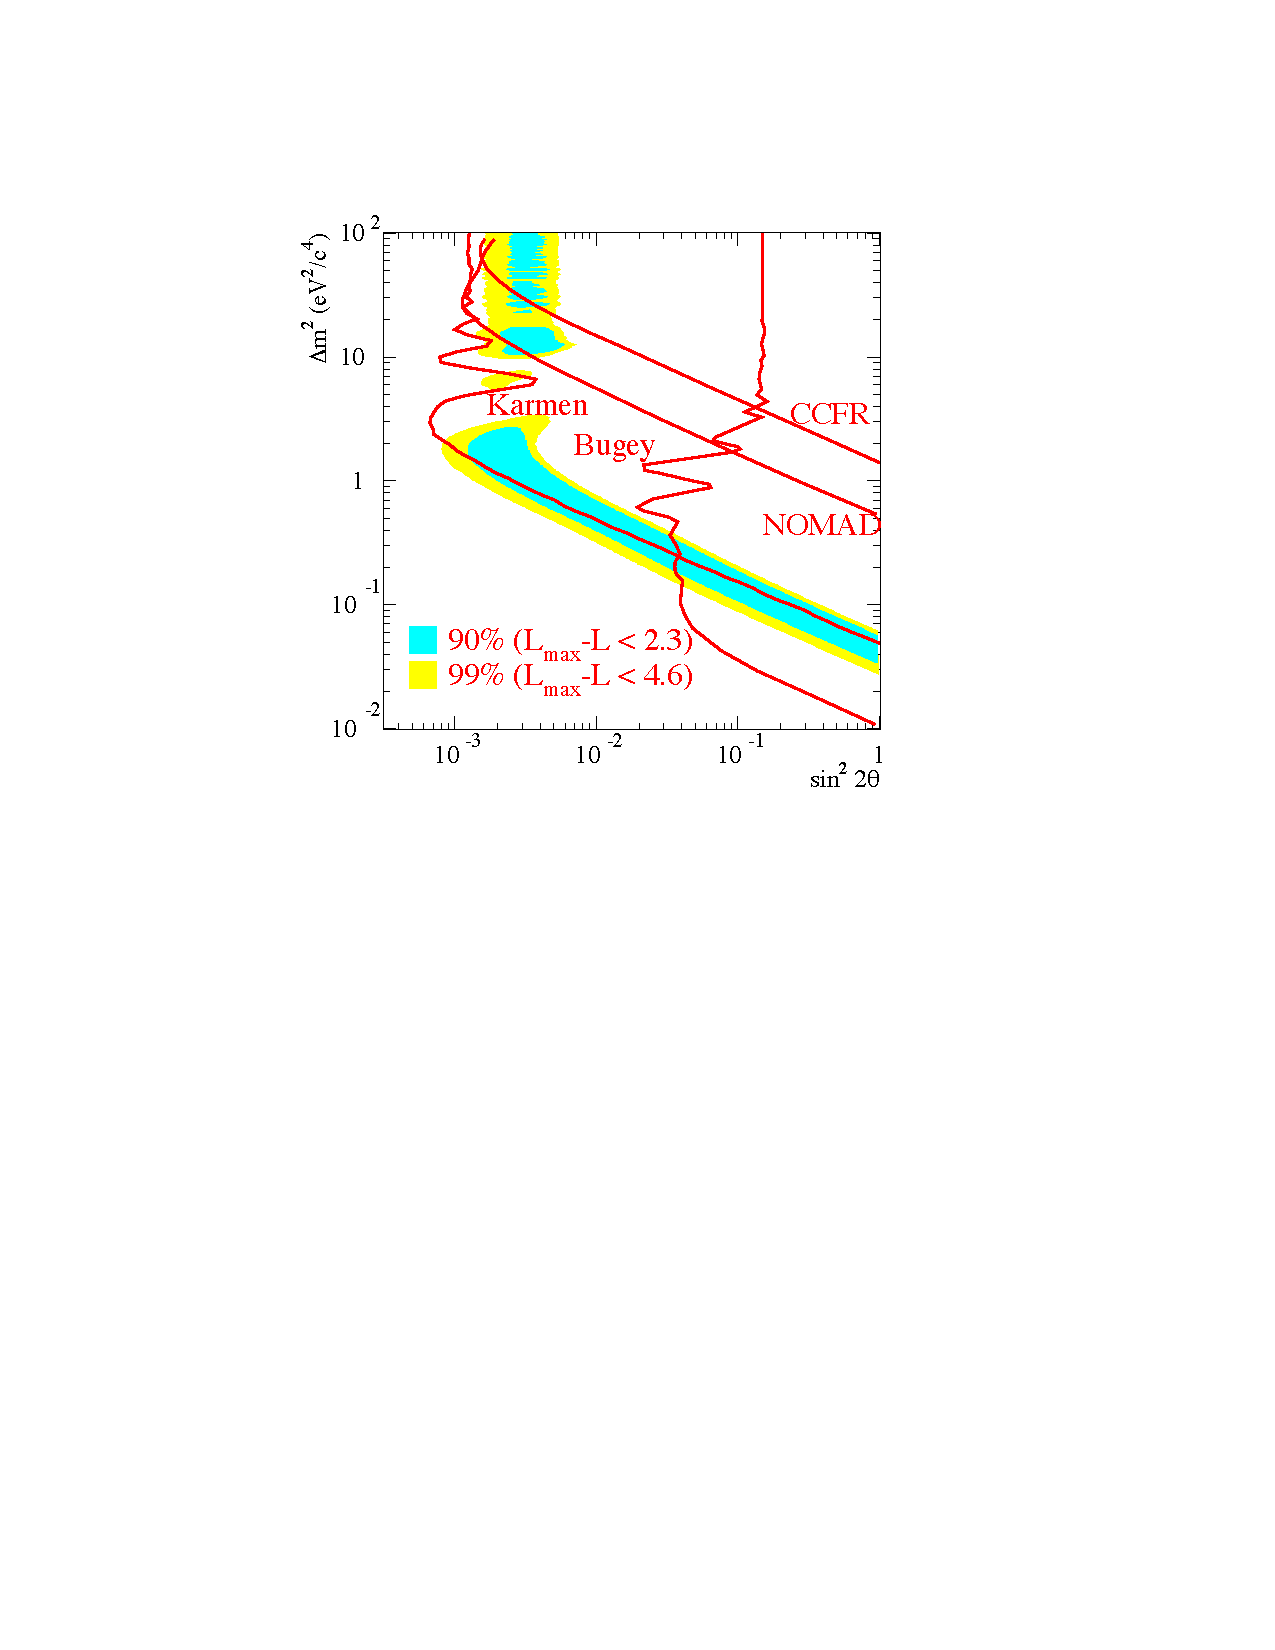
\includegraphics[height=\linewidth]{figures/lsnd_space.pdf}
        \caption{Allowed and excluded regions in the $(\sin^2 2\theta, \Delta m^2)$ parameter space.}\label{fig:lsnd_space}
    \end{center}
  \end{subfigure}
    \caption{The excess of electron antineutrinos observed by the LSND experiment (left) can be interpreted with the presence of a fourth neutrino state. The mixing angles and mass splittings allowed by the LSND data are shown on the right at 90\%~C.L (blue) and 99\%~C.L. (yellow), together with the 90\%~C.L. exclusion limits from other experiments (solid red lines). From \cite{Aguilar:2001ty}.}
\end{figure}

Figure \ref{fig:lsnd_space} shows the regions in the $(\sin^2 2\theta, \Delta m^2)$ parameter space allowed by the LSND data at 90\%~CL and 99\%~CL. %It is possible to identify two mass-splitting terms and three mixing angles, compatible with a scenario of 3 neutrino flavours, while the LSND allowed region is clearly in a completely different region of the parameter space. 
The KARMEN experiment at the Rutherford Appleton Laboratory employed a setup similar to LSND in order to explore the same region, but it found no significant excess and ruled out a large subset of the LSND parameter space \cite{Eitel:2000by}. 

\section{The MiniBooNE experiment}\label{sec:miniboone}
The MiniBooNE experiment was designed to definitely test the LSND result. It consists of a spherical detector filled with mineral oil and located 541 meters downstream of the Booster Neutrino Beam (BNB) production target at Fermilab. This beam can run both in neutrino mode, producing a mainly $\nu_{\mu}$ beam, and in antineutrino mode, producing a mainly $\bar{\nu}_{\mu}$ beam. The BNB neutrino flux is described in detail by the MiniBooNE collaboration in \cite{AguilarArevalo:2008yp} and will be summarised in Section \ref{sec:beam}. The beam energy is one order of magnitude larger than LSND (8 GeV vs. 800 MeV), but the two experiments have a comparable $L/E_{\nu}$ ratio.

The detector is equipped with 1280 8-inch photomultiplier tubes (PMTs) and employs a separated outer veto region with an extra 240 PMTs for cosmic-ray rejection. Particles interacting in the mineral oil produce Cherenkov light, if above production threshold. The particle identification is based on the different light patterns that each particle produces in the detector: in particular, high-penetrating, heavy particles such as muons will produce sharp rings of Cherenkov light, while lighter particles like electrons and photons will produce fuzzier rings. A neutral pion will instead produce two fuzzy rings partially overlapping when it decays to two photons ($\pi^{0}\rightarrow \gamma\gamma$). 
This technique introduces an irreducible degeneracy in the final-state particles, since it is not possible to distinguish a single photon from an electron. Figure \ref{fig:miniboone_evd} shows three MiniBooNE event displays with a muon, an electron (or photon), and a $\pi^0\rightarrow\gamma\gamma$ decay in the final state.

\begin{figure}[htbp]
    \centering
    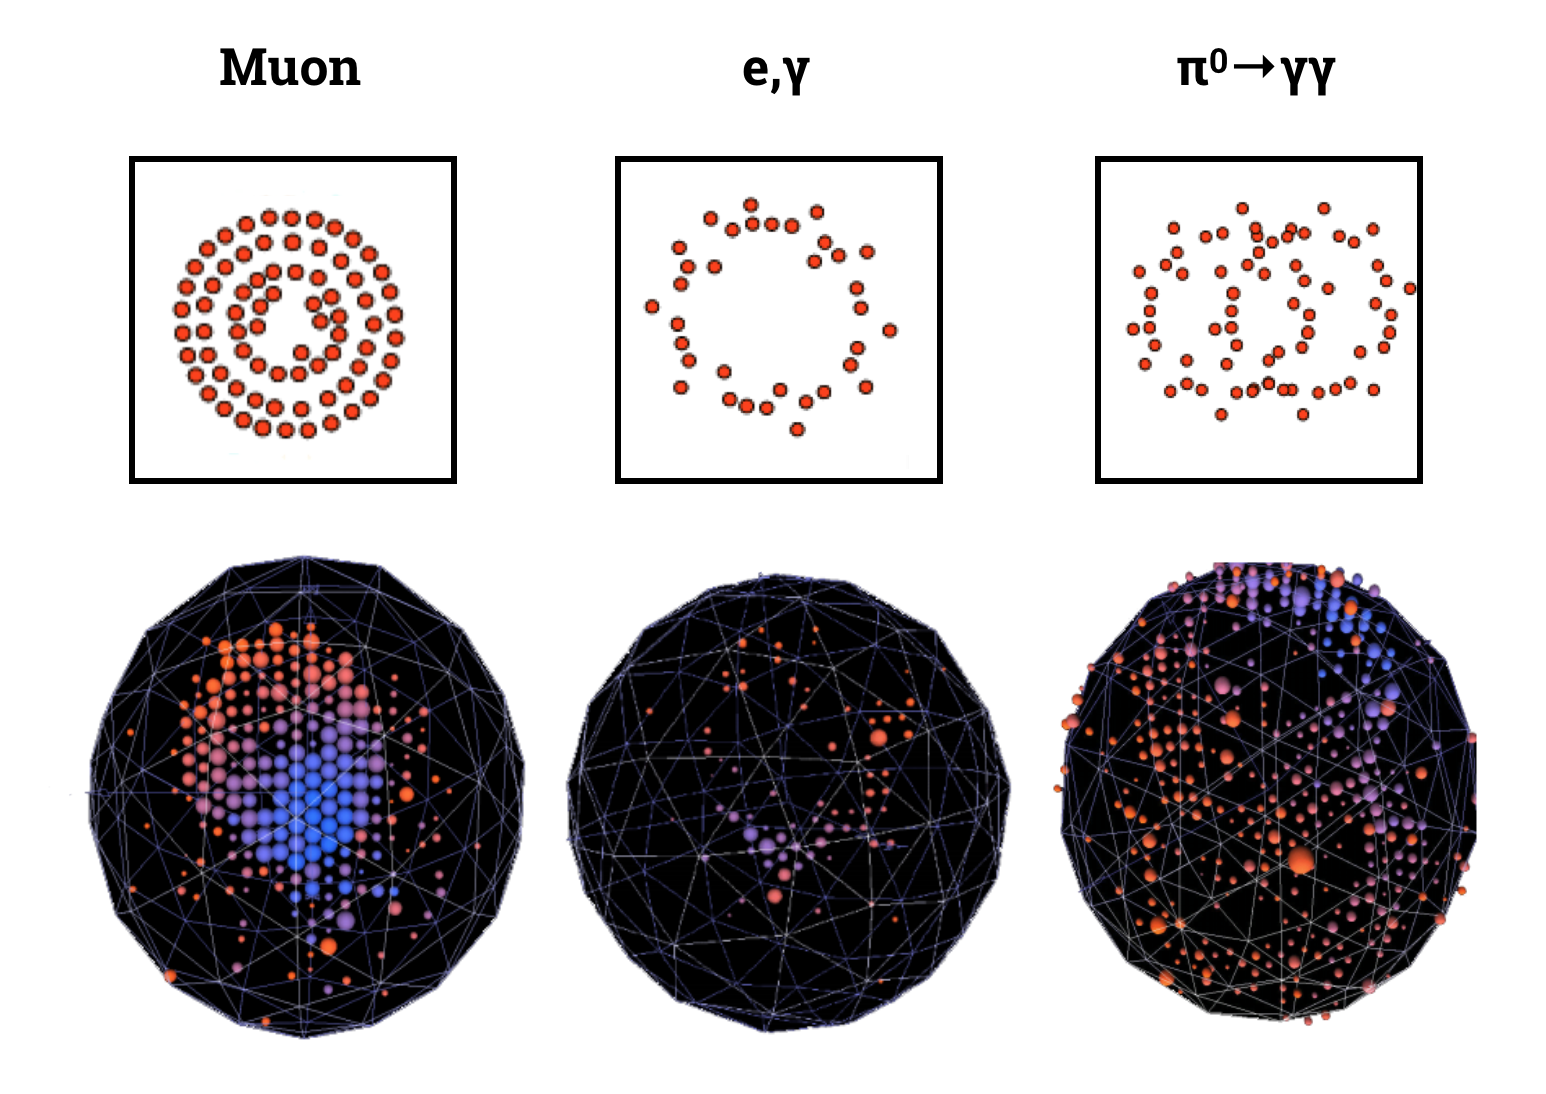
\includegraphics[width=0.85\linewidth]{figures/miniboone_evd.png}
    \caption{Schematics and event display for three topologies in the MiniBooNE detector.}
    \label{fig:miniboone_evd}
\end{figure}

Energy calibration at MiniBooNE was performed with \emph{in situ} measurements. Cosmic muons, detected with an external hodoscope and stopping in the mineral oil, produce the typical Michel electron spectrum peaked at $m_{\mu}/2 = 52.8$~MeV. The invariant mass of $\pi^0$ decays can also be reconstructed to measure the energy response around $135$~MeV. 

The oscillation analysis of the MiniBooNE experiment looked for $\nu_e$ charged-current quasi-elastic (CCQE) interactions, where the $\nu_{e}$ exchanges a charged $W$ boson with a neutron in the nucleus, producing an outgoing electron and a proton. This is the dominant interaction type in the sub-GeV region, as shown in Figure \ref{fig:ccqecross}.

However, as outlined in Section \ref{sec:modes}, FSI can alter the particles produced in the interaction and then detected by the apparatus. In particular, CC1$\pi$ events with pion absorption represent a source of uncertainty for a CCQE analysis, since they share the same particles in the final state.

For this reason, in MiniBooNE, the selected events are called \emph{CCQE-like}, since this definition relies only on the particles in the final state \cite{Katori:2013nca}. 

The energy of the CCQE-like interaction $E_{\nu}^{QE}$ is determined by the electron scattering angle $\theta$ and energy $E_e$, assuming the nucleon at rest, as:
\begin{equation}
    E_{\nu}^{QE} = \frac{2m_n E_e + m_p^2- m_n^2 - m_e^2}{2(m_n - E_e + \cos\theta\sqrt{E_e^2-m_e^2})},\label{eq:ccqe}
\end{equation}
where $m_n$, $m_p$, and $m_e$ are the mass of the neutron, the proton, and the electron, respectively. 
In reality, the nucleon will have a certain Fermi momentum, which will smear out the reconstructed energy. In this case, the estimation of the neutrino energy will depend on the particular model of Fermi motion employed in the simulation, introducing a systematic uncertainty in the measurement.

The presence of events with pion absorption or where the pion escapes the detector introduces as well a distortion in the energy distribution, since the approximation of a 2-body interaction of Equation \ref{eq:ccqe} is no longer valid.


\begin{figure}[htbp]
  \begin{subfigure}{0.48\textwidth}
    \begin{center}
    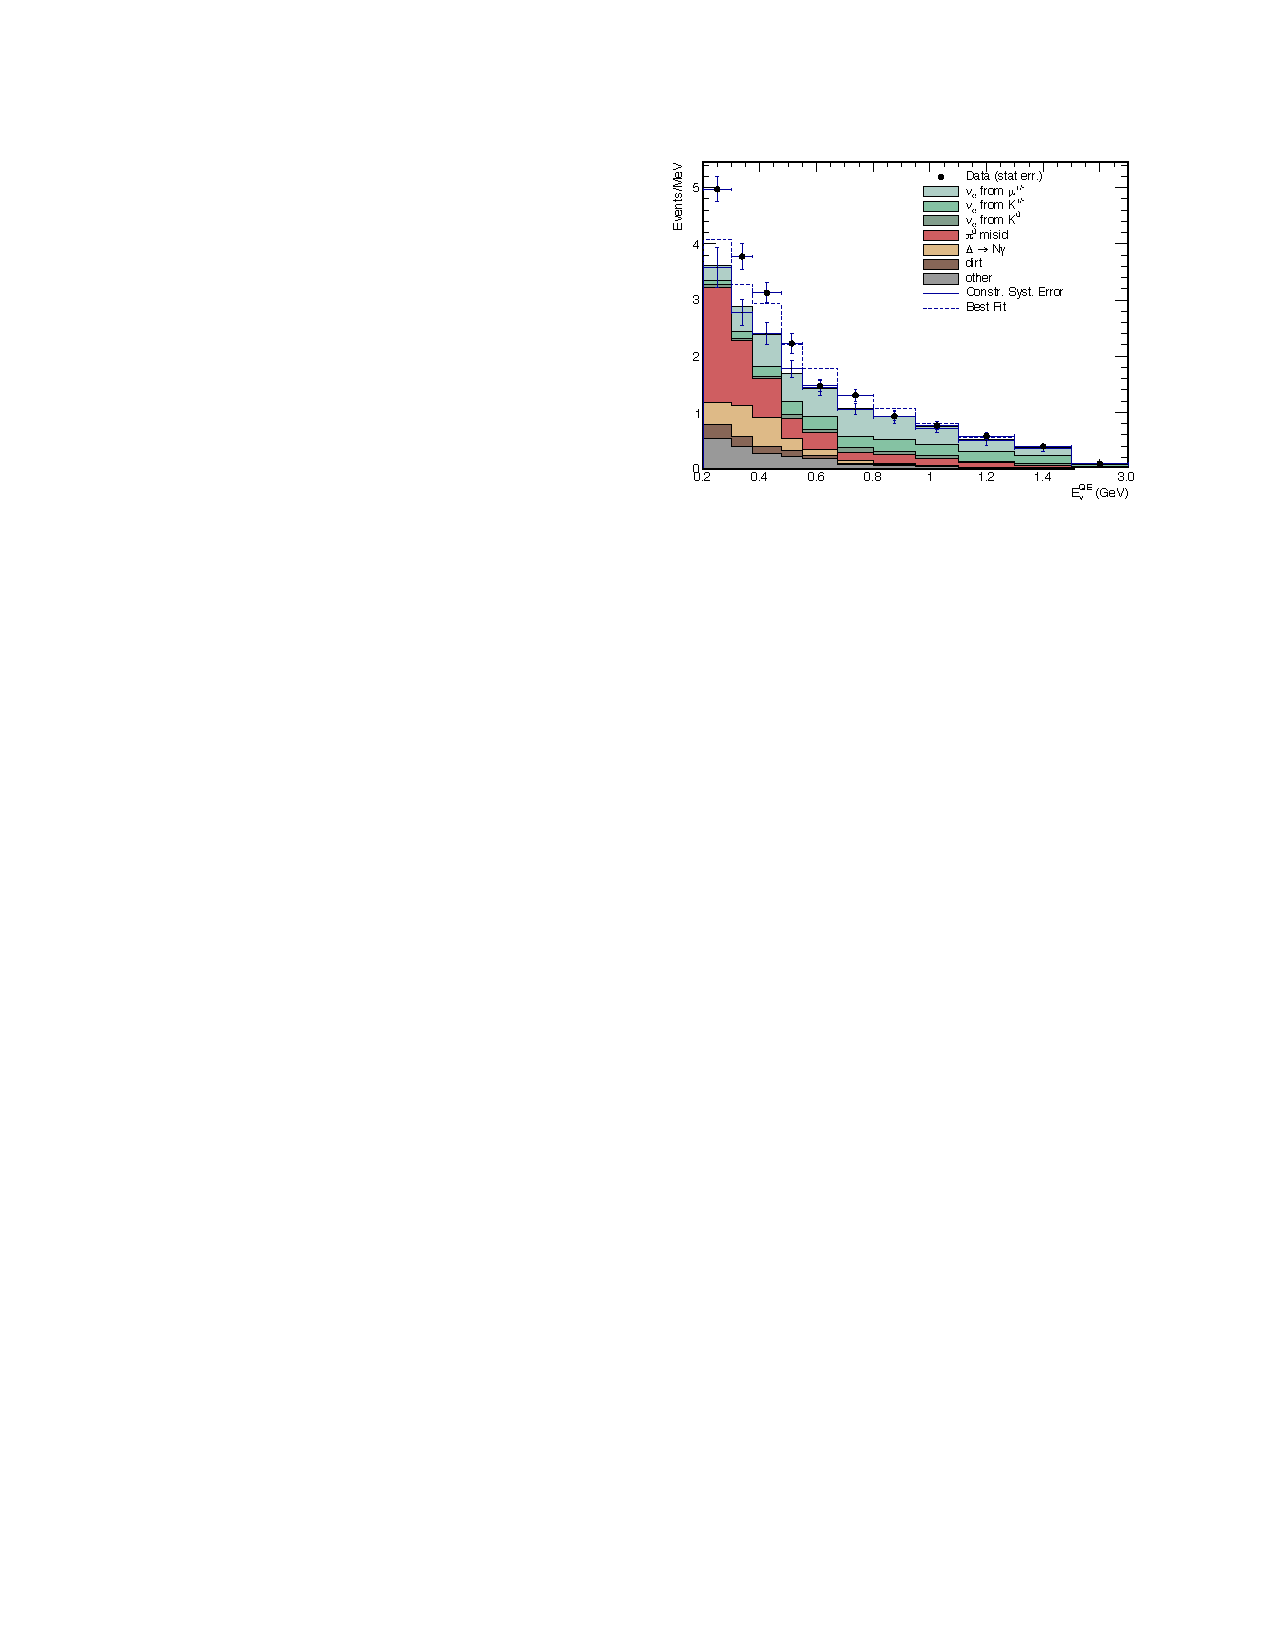
\includegraphics[width=\linewidth]{figures/miniboone_plot.pdf}
    \caption{$E_{\nu}^{QE}$ spectrum in neutrino mode.}
    \label{fig:miniboone_spectrum}
    \end{center}
  \end{subfigure}\hfill
  \begin{subfigure}{0.48\textwidth}
    \begin{center}
    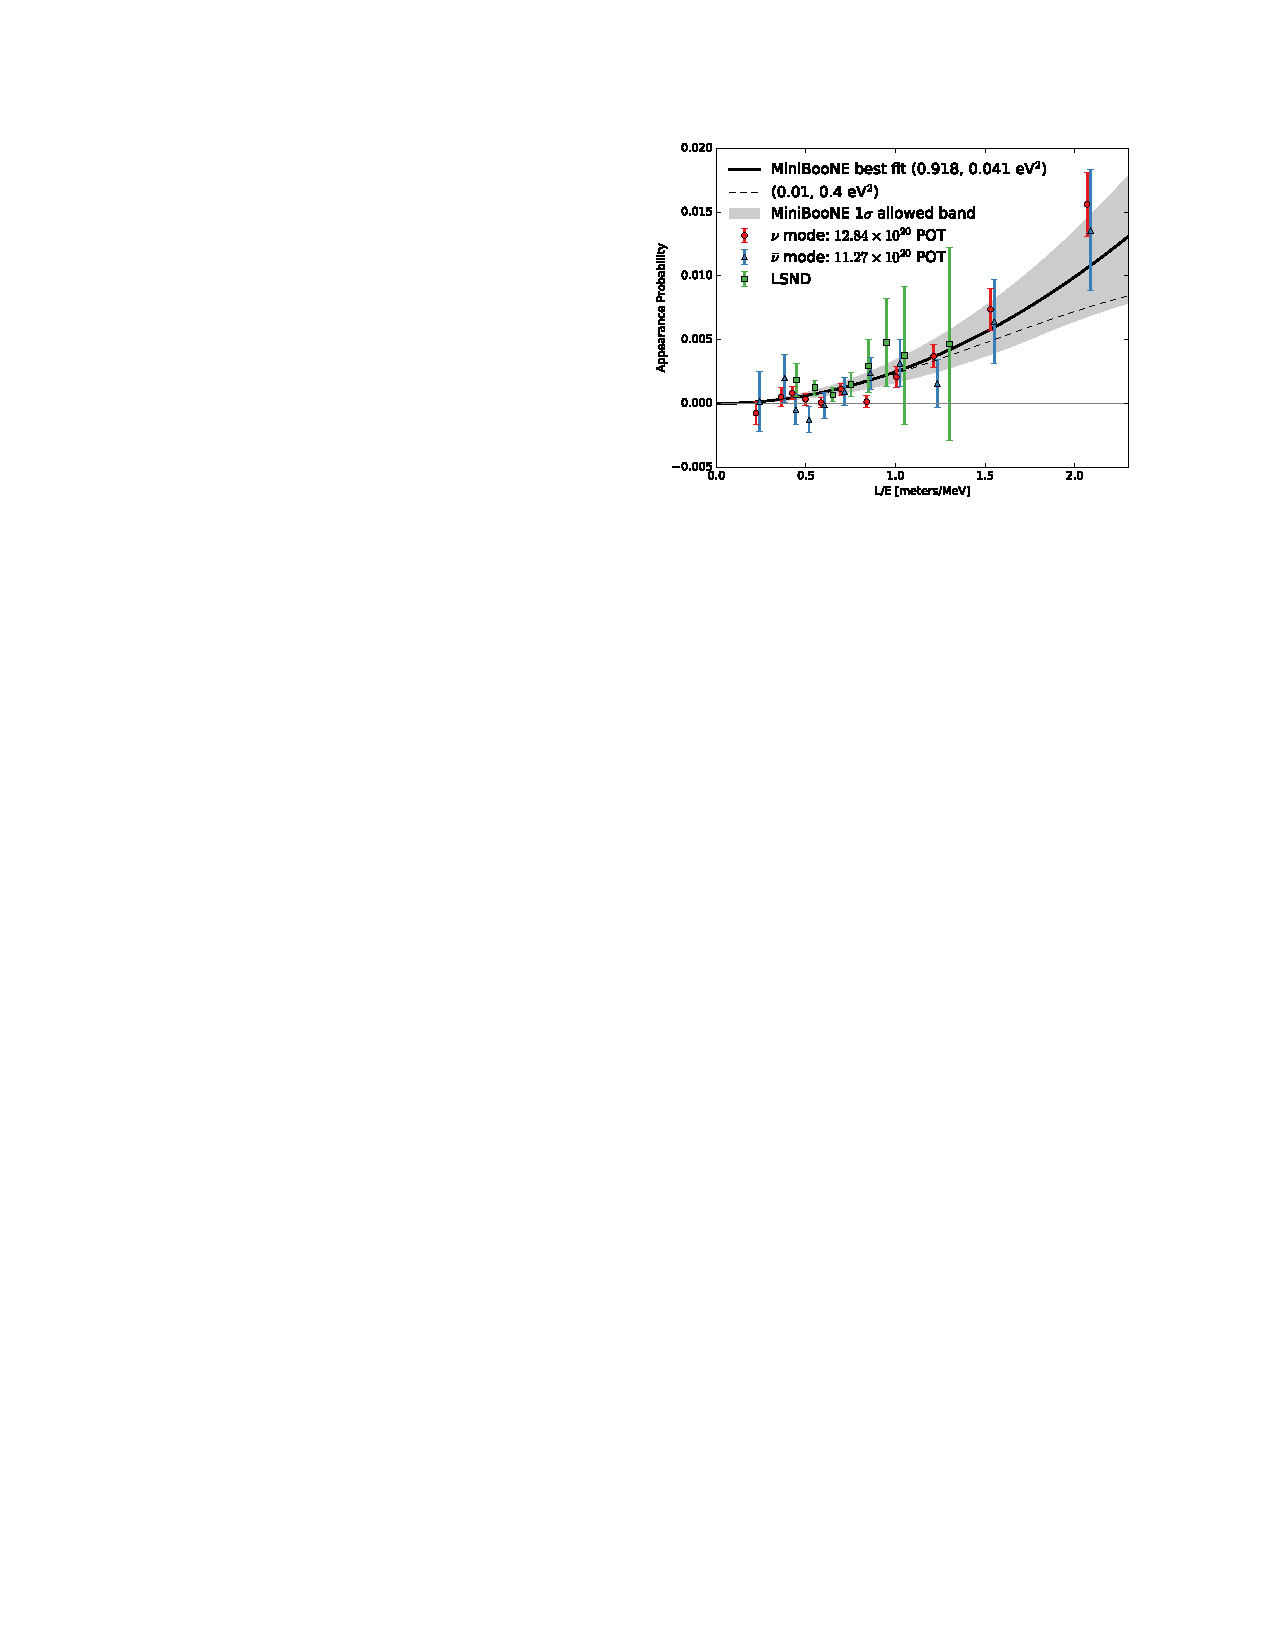
\includegraphics[width=\linewidth]{figures/miniboone_lsnd.pdf}
    \caption{Appearance probability.}
    \label{fig:miniboone_lsnd}
    \end{center}
  \end{subfigure}
  \caption{The MiniBooNE neutrino mode corresponding to the total $12.84\times10^{20}$ POT data, for $\nu_e$ CCQE data (points with statistical errors) and background (histogram with systematic errors). The dashed line represent the two-neutrino model best fit (left). The appearance probability as a function of the $L/E$ ratio is in agreement with LSND data (right). Adapted from \cite{Aguilar-Arevalo:2018gpe}.}
\end{figure}


The most recent result by the MiniBooNE collaboration \cite{Aguilar-Arevalo:2018gpe} shows a $4.7\sigma$ excess in the combined $\nu_{e}$ and $\bar{\nu}_{e}$ analysis, for $12.84\times10^{20}$ ($11.27\times10^{20}$) POT collected in neutrino (antineutrino) mode. The observed excess of data events is $460.5 \pm 99.0$. The energy spectrum of the $\nu_E^{\mathrm{CCQE}}$ selected events in neutrino mode is shown in Figure \ref{fig:miniboone_spectrum}. The analysis followed a blind approach, where the data sub-sample containing the signal events, defined requiring a single isolated electron in the detector, was not opened until the analysis tools and the simulation were well understood. 

The $\nu_{e}$ oscillation was measured with a combined fit of the $\nu_{e}$ and $\nu_{\mu}$ selected events. This approach, which will be employed also by the MicroBooNE experiment, allows to measure more precisely the neutrino flux: in this way, the $\nu_e$ candidates from $\nu_{\mu}$ oscillation cannot be interpreted as an underestimation of the total neutrino flux, since this would show up as a disagreement in the number of $\nu_{\mu}$ events as well. A measurement of the $\nu_{\mu}$ component of the flux allows also to partially constrain the number of intrinsic $\nu_e$ since around half of them are produced in the decay:
\begin{align}
    \pi^+ \rightarrow & \mu^+\nu_{\mu}\\
    & \rotatebox[origin=c]{180}{$\Lsh$}	 \mu^{+} \rightarrow e^+\bar{\nu}_{\mu}\nu_{e}.
\end{align}

The excess of data events is in the sub-GeV energy region and is consistent in energy and magnitude with the LSND result. The two excess combined give a significance of $6.0\sigma$. Figure \ref{fig:miniboone_lsnd} shows the agreement of the appearance probability as a function of the $L/E_{\nu}$ distribution for LSND and MiniBooNE. 

\subsection*{MiniBooNE backgrounds}
The background events of the MiniBooNE experiment can be divided into four main categories:
\begin{description}
    \item[Intrinsic $\nu_e$.] The $\nu_e$ component of the beam, coming from $\mu^{\pm}$, $K^{\pm}$, and $K^0$, is the irreducible background of the experiment, since it can't be distinguished from $\nu_{\mu}$ oscillating into $\nu_{e}$. This component of the flux is partially constrained by measuring the $\nu_{\mu}$ interactions.
    \item[Misidentified $\pi^0$.] The background from misidentified $\pi^0$ events represents the largest component. These events are particularly challenging to reconstruct since very forward-boosted photons will appear in the detector as a single fuzzy ring. The MiniBooNE collaboration has constrained this contribution by reconstructing the invariant $\pi^0$ mass of the event and obtaining a sample with a purity $>90\%$ of NC $\pi^0$ events. The total uncertainty on the NC background is 7\% \cite{Karagiorgi:2010zz}.
    \item[Misidentified $\Delta\rightarrow N\gamma$.] A neutral current resonant interaction can produce a $\Delta$ resonance, which has a rare electromagnetic decay channel $\Delta\rightarrow N\gamma$, where $N=n,p$. This channel is also constrained by the NC $\pi^0$ \emph{in situ} measurement, times the small branching ratio  $(0.56\pm0.04)\%$. The uncertainty on this component is 12\%.
    \item[Dirt.] The dirt background, meaning neutrino interactions happening outside the detector but where at least one particle in the final states interacts inside, is also constrained with an \emph{in situ} measurement, where events reconstructed close to the detector boundaries and pointing inwards are selected. 
\end{description}

Both the $\pi^0$ and the $\Delta\to N\gamma$ backgrounds come from the inability of a Cherenkov detector to distinguish between photons and electrons, which is instead one of the most powerful capabilities of a LArTPC, as it will be described in detail in Section \ref{sec:detector}. MiniBooNE is also not able to distinguish between negative and positive charged particles, making it impossible to distinguish between neutrino and antineutrino events.

Non-beam backgrounds (such as cosmic rays) are removed by requiring light in the detector in time with the BNB spill of 1.6~\si{\micro}s and no activity in the outer veto volume, achieving a 99.99\% rejection efficiency. 
In order to reject the beam-related background events, the MiniBooNE collaboration employed an electron-muon likelihood cut, an electron-pion likelihood cut, and a cut on the invariant $m_{\gamma\gamma}$ mass.

The average selection efficiency for $\nu_e^{\mathrm{CCQE}}$ events is $\sim20$\% \cite{Aguilar-Arevalo:2018gpe}.

\subsection*{Possible interpretations of the LSND and MiniBooNE results}

A proposed solution to the LSND anomaly is to have one sterile additional neutrino state, which would mix with the standard three neutrinos, in a (3+1) scenario. The PMNS matrix, in this case, will have an extra dimension ($4\times4$) and the sterile mass neutrino eigenstate will be written as:
\begin{equation}
    \ket{\nu_s}=\sum^{3+1}_{\alpha}U_{i,\alpha}\ket{\nu_{\alpha}}.
\end{equation}
A diagram of the mass hierarchy in this scenario is available in Figure \ref{fig:masslsnd}.

\begin{figure}[htbp]
    \centering
    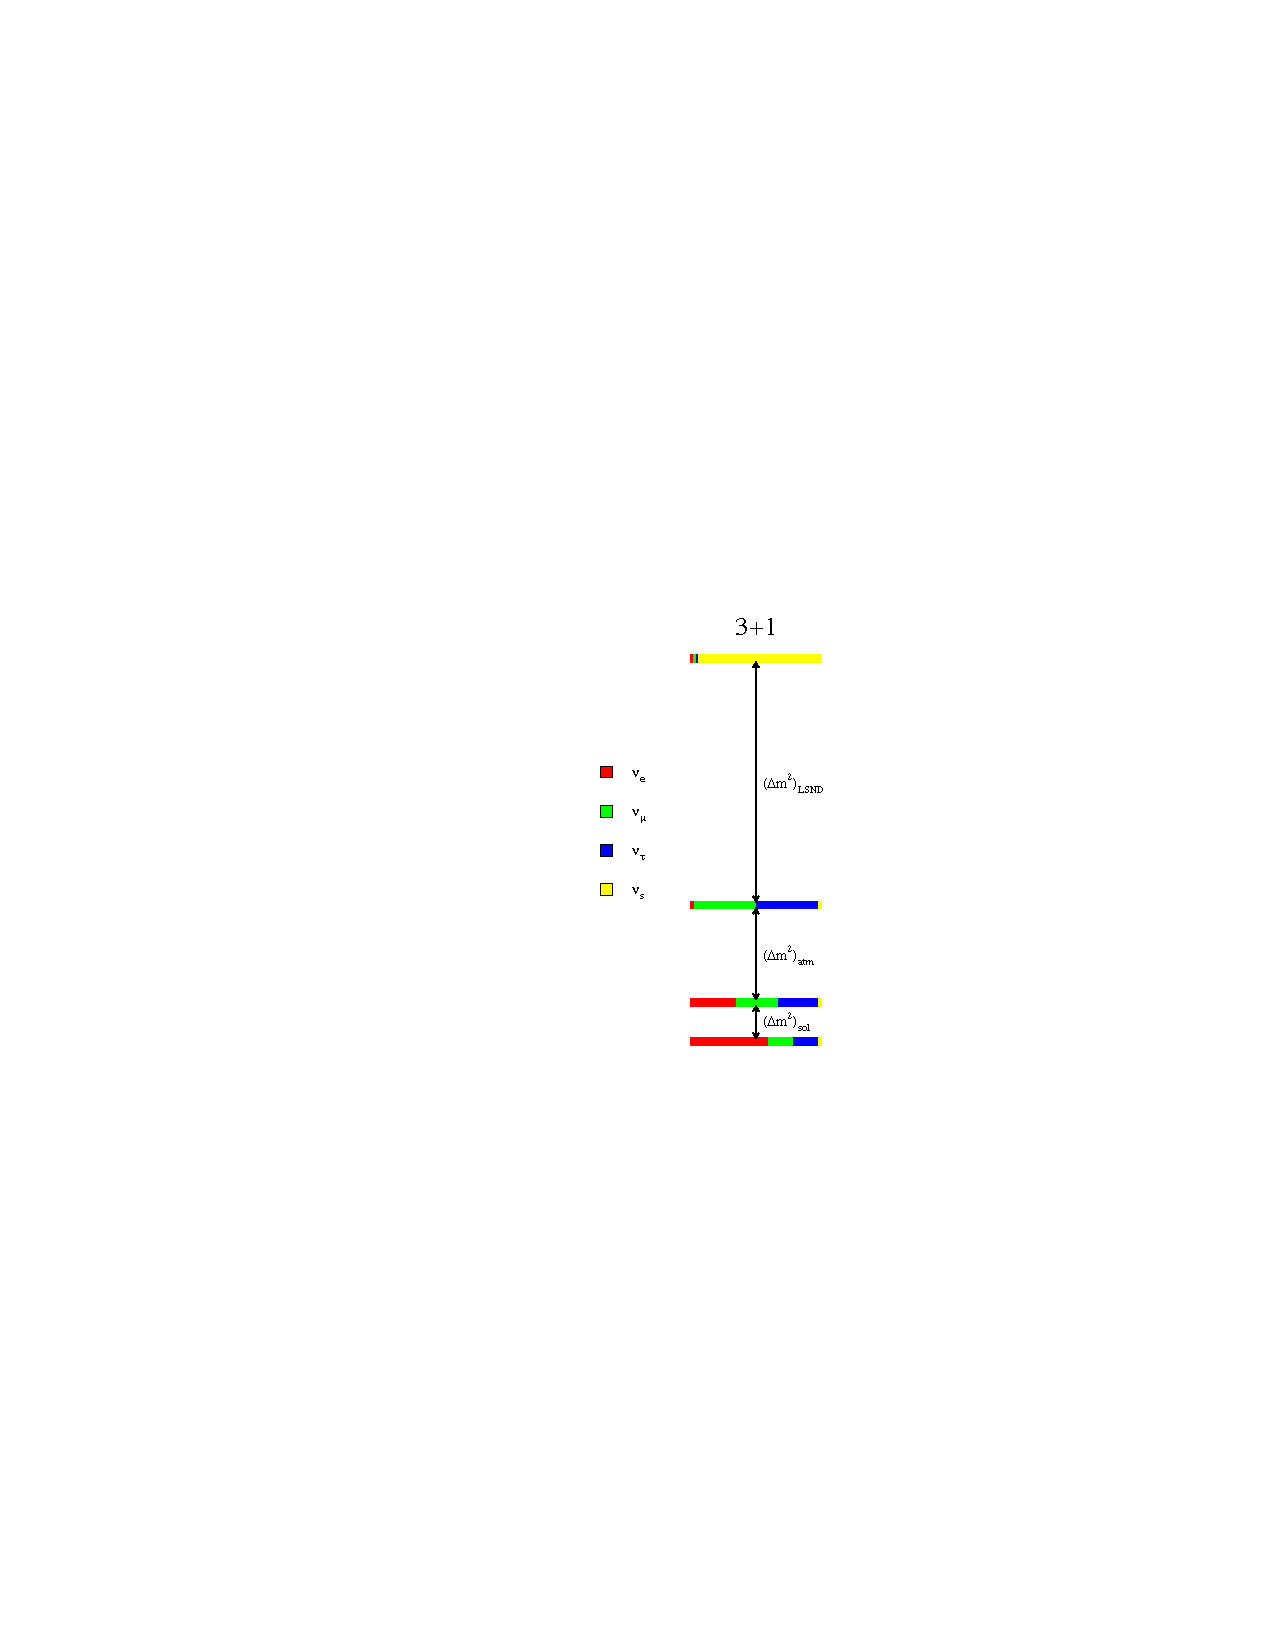
\includegraphics[width=0.3\linewidth]{figures/masslsnd.pdf}
    \caption{Neutrino mass normal hierarchy in the scenario of 3+1 neutrinos (from \cite{deGouvea:2004gd}).}
    \label{fig:masslsnd}
\end{figure}

As shown in Figure \ref{fig:miniboone_lsnd}, the LSND excess seems to be in agreement with the results of the MiniBooNE experiment, both in neutrino and antineutrino mode. The MiniBooNE collaboration was able to constrain all the simulated experimental backgrounds with \emph{in situ} measurements. The excess must then come from an unexpected background source or from BSM interactions, such as the existence of one or more sterile neutrinos.
Figure \ref{fig:miniboone_bestfit} shows the MiniBooNE allowed regions in neutrino and antineutrino mode for the two-neutrino oscillation model. The best-fit point, however, is disfavoured by the OPERA $\nu_{e}$ appearance analysis \cite{Agafonova:2018dkb}.

\begin{figure}[htbp]
    \centering
    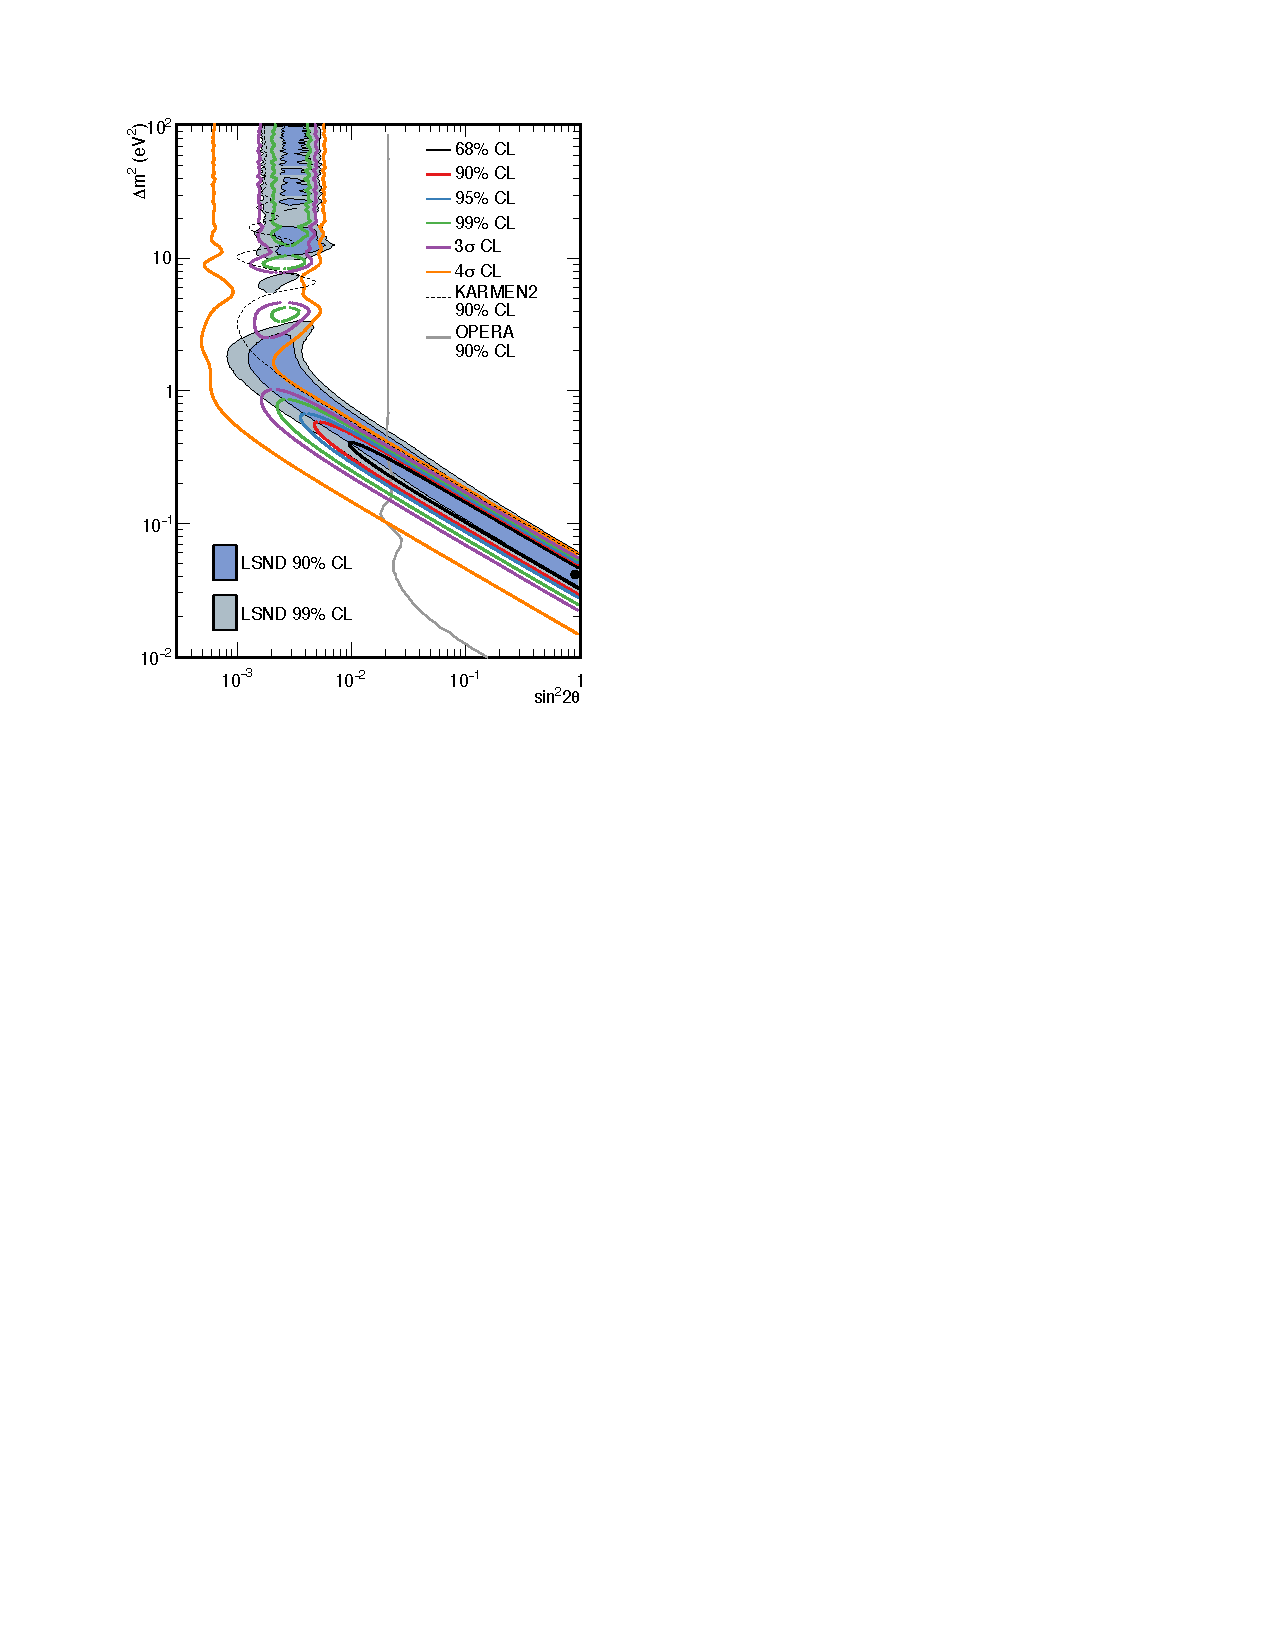
\includegraphics[width=0.7\linewidth]{figures/miniboone_bestfit.pdf}
    \caption{MiniBooNE allowed regions for the combined neutrino mode and antineutrino for events with $200<E_{\nu}^{QE}<3000$~MeV within a two-neutrino oscillation model. The black point at $( \sin^22\theta, \Delta m^2)=(0.96, 0.041~\mathrm{eV^2})$ represents the best fit \cite{Aguilar-Arevalo:2018gpe}.}
    \label{fig:miniboone_bestfit}
\end{figure}


\section{Oscillations anomalies: the global picture}
The global fit of neutrino oscillations experiments in the 2-neutrino approximation (so using Equations \ref{eq:prob} and \ref{eq:prob2}) is shown in Figure \ref{fig:globalfit}. Atmospheric, solar, and reactor experiments roughly overlap in three regions in the $(\tan^2\theta, \Delta m^2)$ space, giving three mixing angles and two mass splittings values, as expected in a 3-flavour scenario. 

\begin{figure}[htbp]
    \centering
    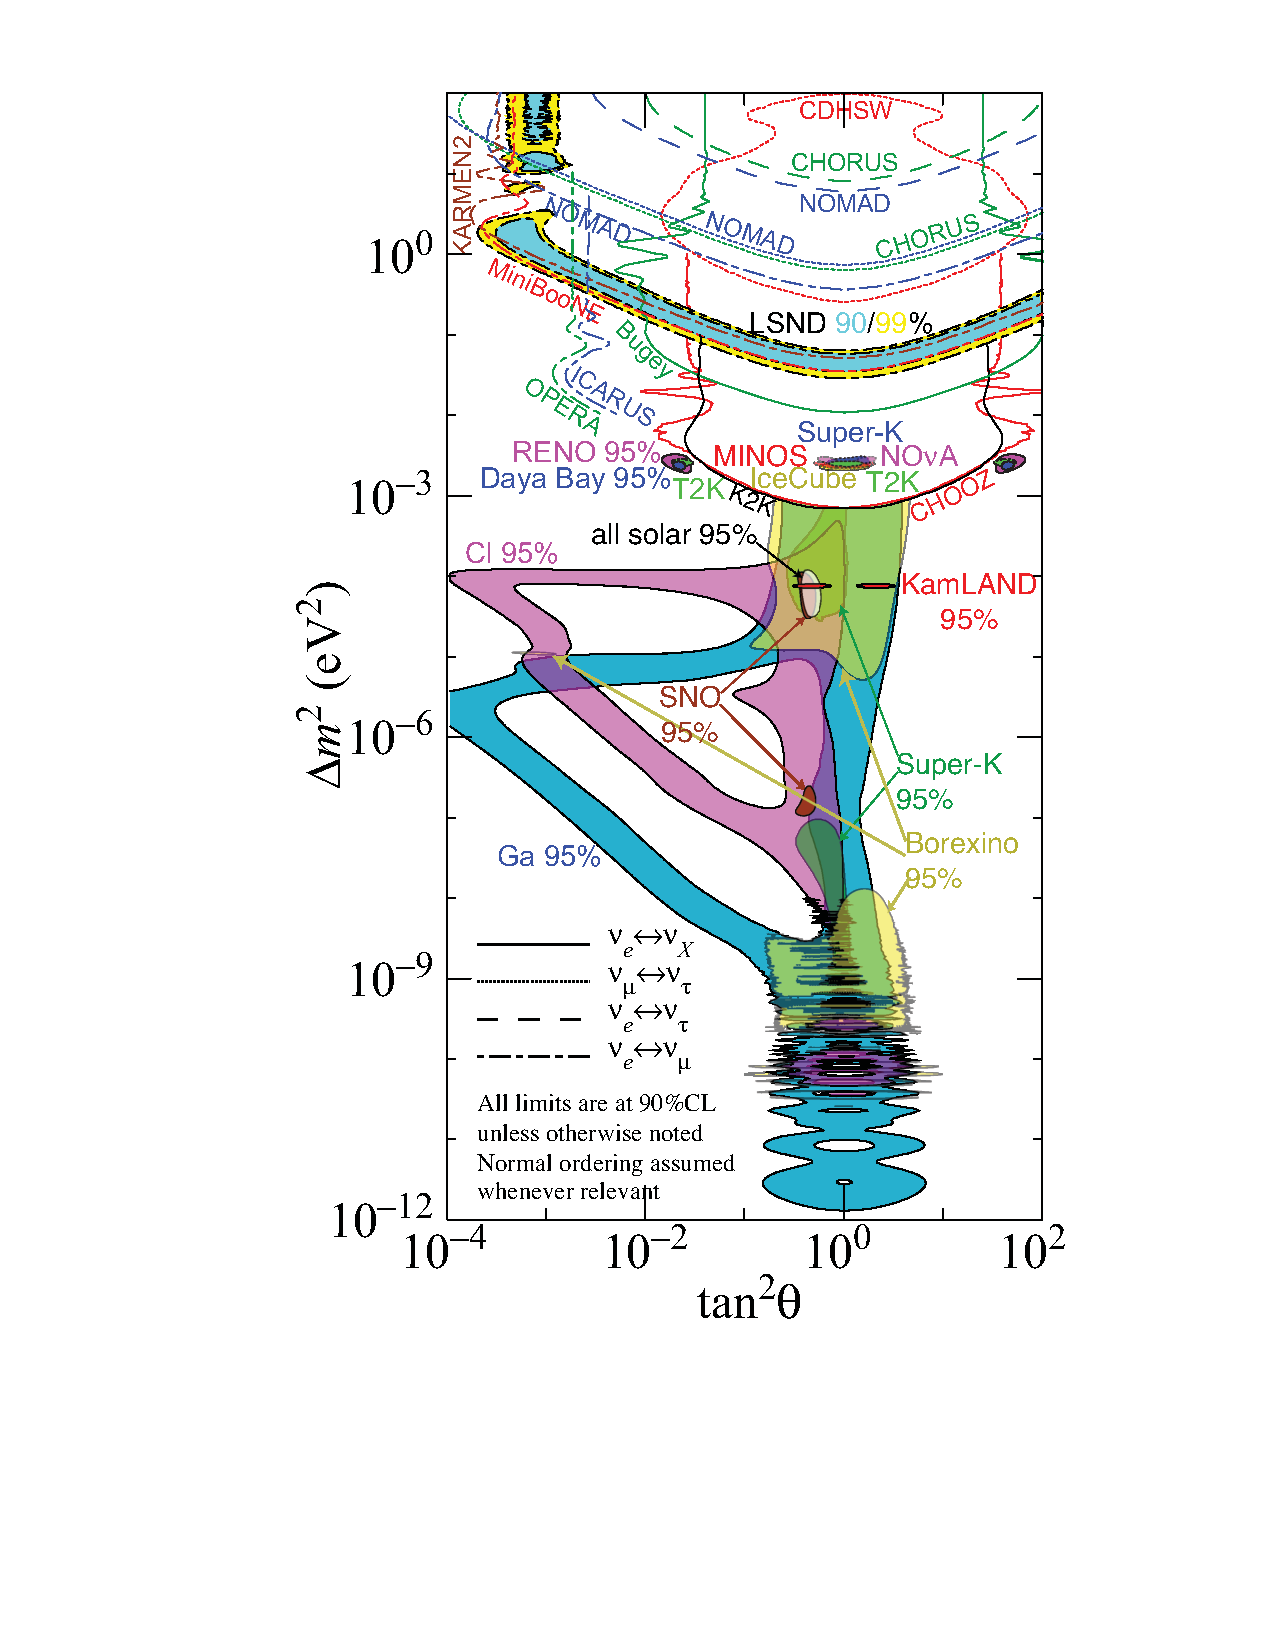
\includegraphics[width=0.7\linewidth]{figures/globalfit.pdf}
    \caption{The squared-mass splittings and mixing angles favoured (solid regions) or excluded (open regions) by existing neutrino oscillation measurements. Results are categorised by channels: $\nu_e$ disappearance (solid lines), $\nu_{\mu} \leftrightarrow \nu_{\tau}$  (dotted lines), $\nu_{e} \leftrightarrow \nu_{\tau}$ (dashed lines), and $\nu_{e} \leftrightarrow \nu_{\mu}$ (dashed-dotted lines). The normal mass ordering is assumed where relevant. Taken from \cite{PhysRevD.98.030001}. Does not include MiniBooNE latest result \cite{Aguilar-Arevalo:2018gpe}.}
    \label{fig:globalfit}
\end{figure}

However, LSND and MiniBooNE results do not agree with the allowed regions since their mass splitting term is much larger ($\Delta m^2 \approx1~$eV$^2$). Moreover, they are not the only two experiments to have observed anomalies in the neutrino sector. Several other experiments obtained results not completely in agreement with the theoretical expectations. In particular, it is possible to identify two categories of anomalies, classified according to the experimental technique employed: inverse beta decay from solar neutrinos of gallium into germanium (\emph{radiochemical experiments}) and inverse beta decay from reactor neutrinos (\emph{reactor experiments}).

\subsection{Radiochemical experiments}
    The GALLEX experiment at Gran Sasso and the SAGE experiment at Baksan employed a detection technique similar to the one of Ray Davis experiment at Homestake. In this case, solar neutrino interactions were detected through inverse $\beta$ decay of $^{71}$Ga atoms into $^{71}$Ge (instead of $^{37}$Cl into $^{37}$Ar at Homestake):
\begin{equation}
    \nu_e + ^{71}\mathrm{Ga} \rightarrow e^- + ^{71}\mathrm{Ge}.
\end{equation}
The energy threshold for this reaction is 233~keV, which allows to observe the neutrino interactions produced in the solar $pp$ chain reaction (see Figure \ref{fig:solar}). Both experiments employed intense radioactive sources for calibration. GALLEX used a $^{51}$Cr source, while SAGE used $^{51}$Cr and $^{37}$Ar. These two sources decay via electron capture, emitting an electron neutrino:
\begin{equation} 
    ^{A}_{Z}\mathrm{X} + e^{-} \rightarrow ^{A}_{Z-1}\mathrm{Y} + \nu_{e}.
\end{equation}

The two experiments observed a deficit of $\nu_{e}$ interactions in all the three cases, which favours with $2.7\sigma$ significance the hypothesis of short-baseline neutrino oscillation \cite{Giunti:2010zu}.

\begin{figure}[htbp]
  \begin{subfigure}{0.48\textwidth}
    \begin{center}
    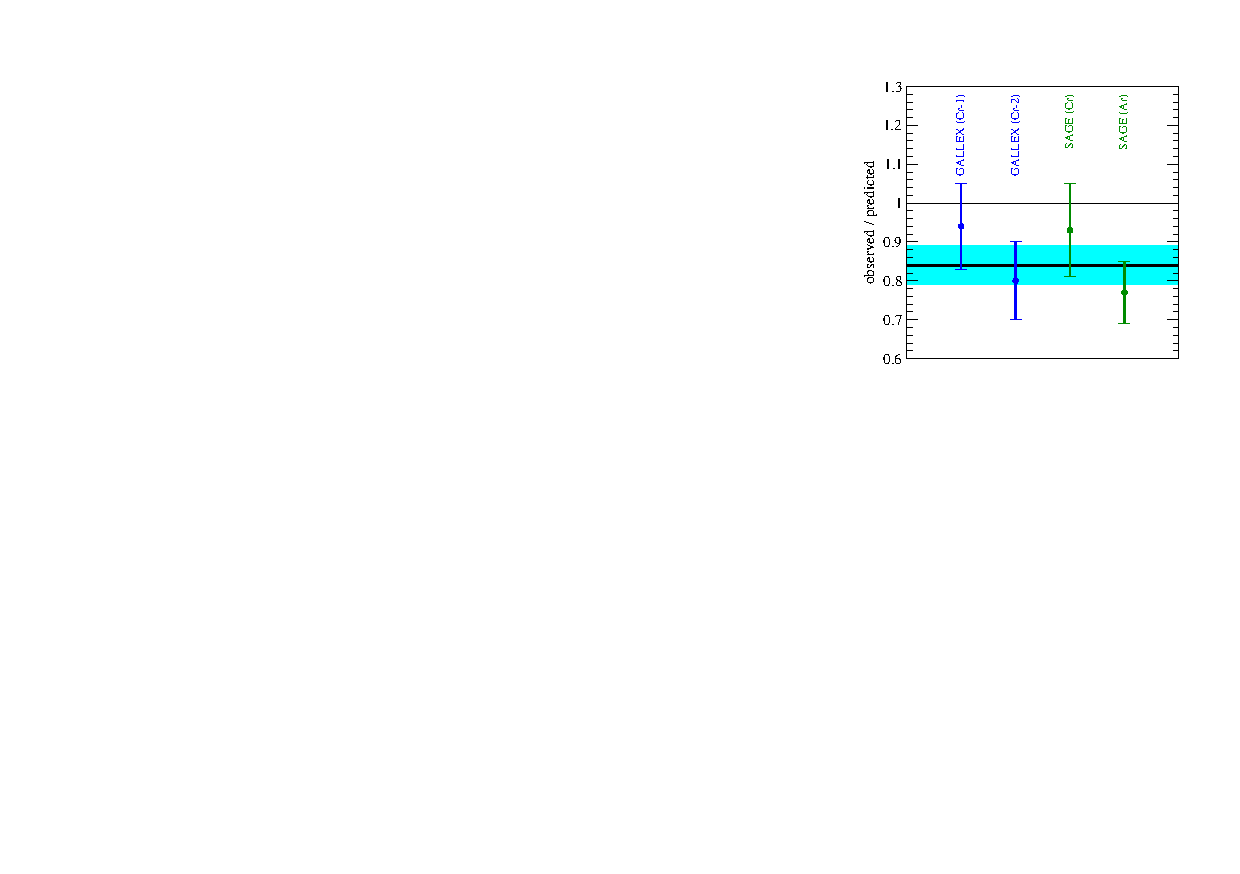
\includegraphics[width=\linewidth]{figures/radiochemical_ratio.pdf}
    \caption{Observed / predicted ratio of $\nu_e$ interactions.}
    \end{center}
  \end{subfigure}\hfill
  \begin{subfigure}{0.48\textwidth}
    \begin{center}
    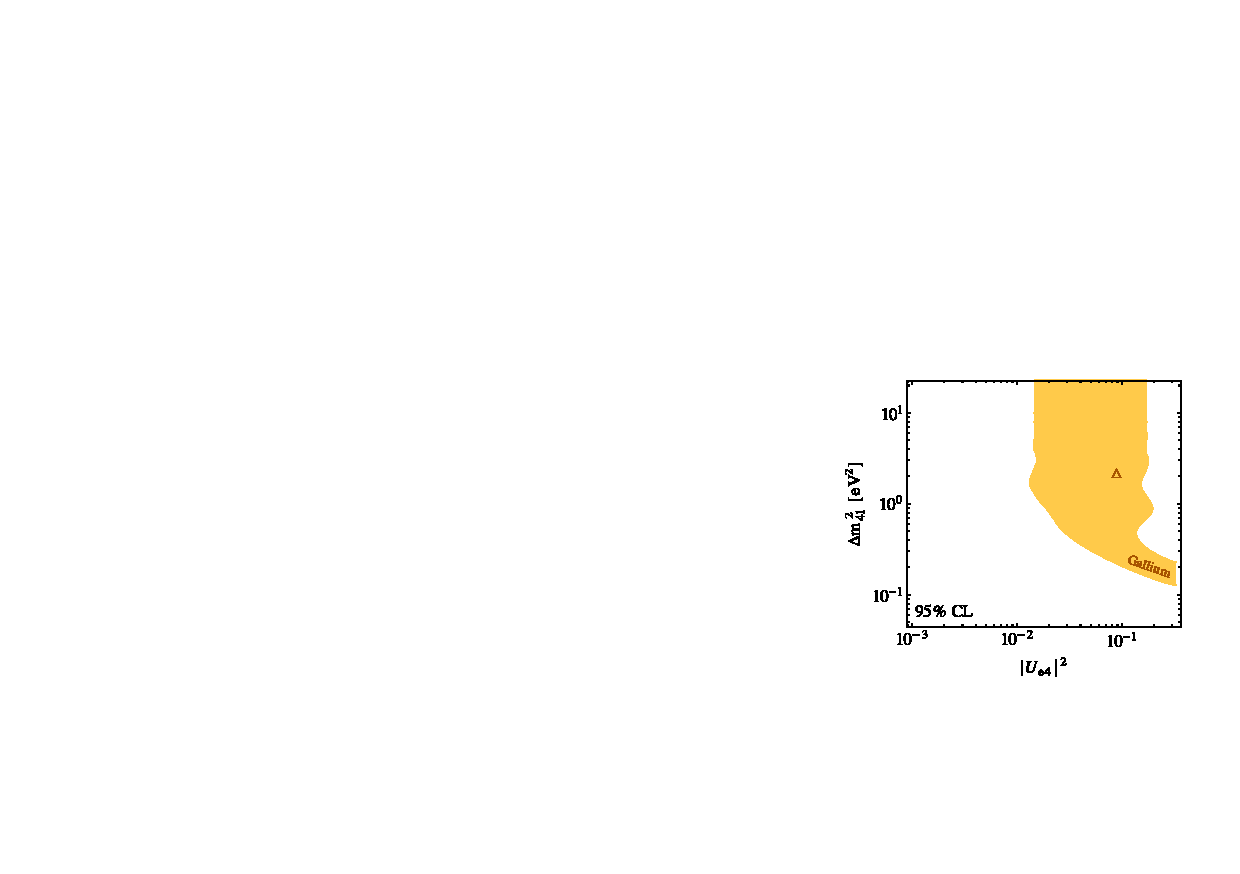
\includegraphics[width=\linewidth]{figures/radiochemical_space.pdf}
    \caption{Allowed parameter space for sterile neutrino oscillation.}
    \end{center}
  \end{subfigure}
  \caption{The SAGE and GALLEX experiments observed a deficit of electron neutrino interactions using radioactive isotopes, which could be explained by introducing oscillations into a sterile neutrino state.}\label{fig:radiochemical}
\end{figure}

Figure \ref{fig:radiochemical} shows the deficit for the four calibration runs (two with $^{51}$Cr for GALLEX, one with $^{51}$Cr and one with $^{37}$Ar for SAGE) and the allowed parameter space in the case of sterile neutrino oscillations in the (3+1) model.

Curiously, during the second data-taking run of SAGE, 2 tons of gallium were stolen from the detector (3.6\% of the total mass) \cite{Abdurashitov:1999zd}.
    
\subsection{Reactor experiments} 
Several reactor neutrino experiments have measured a deficit of events in the antineutrino spectra. This anomaly first appeared in 2011, when an improved calculation of the reactor antineutrino spectra was made available \cite{Mueller:2011nm}. Historical data from several reactor experiments, which before the recalculation were in agreement with the theoretical predictions, all showed a $\sim6\%$ deficit in the spectra, as shown in Figure \ref{fig:reactor}. 
    
    \begin{figure}[htbp]
      \centering
      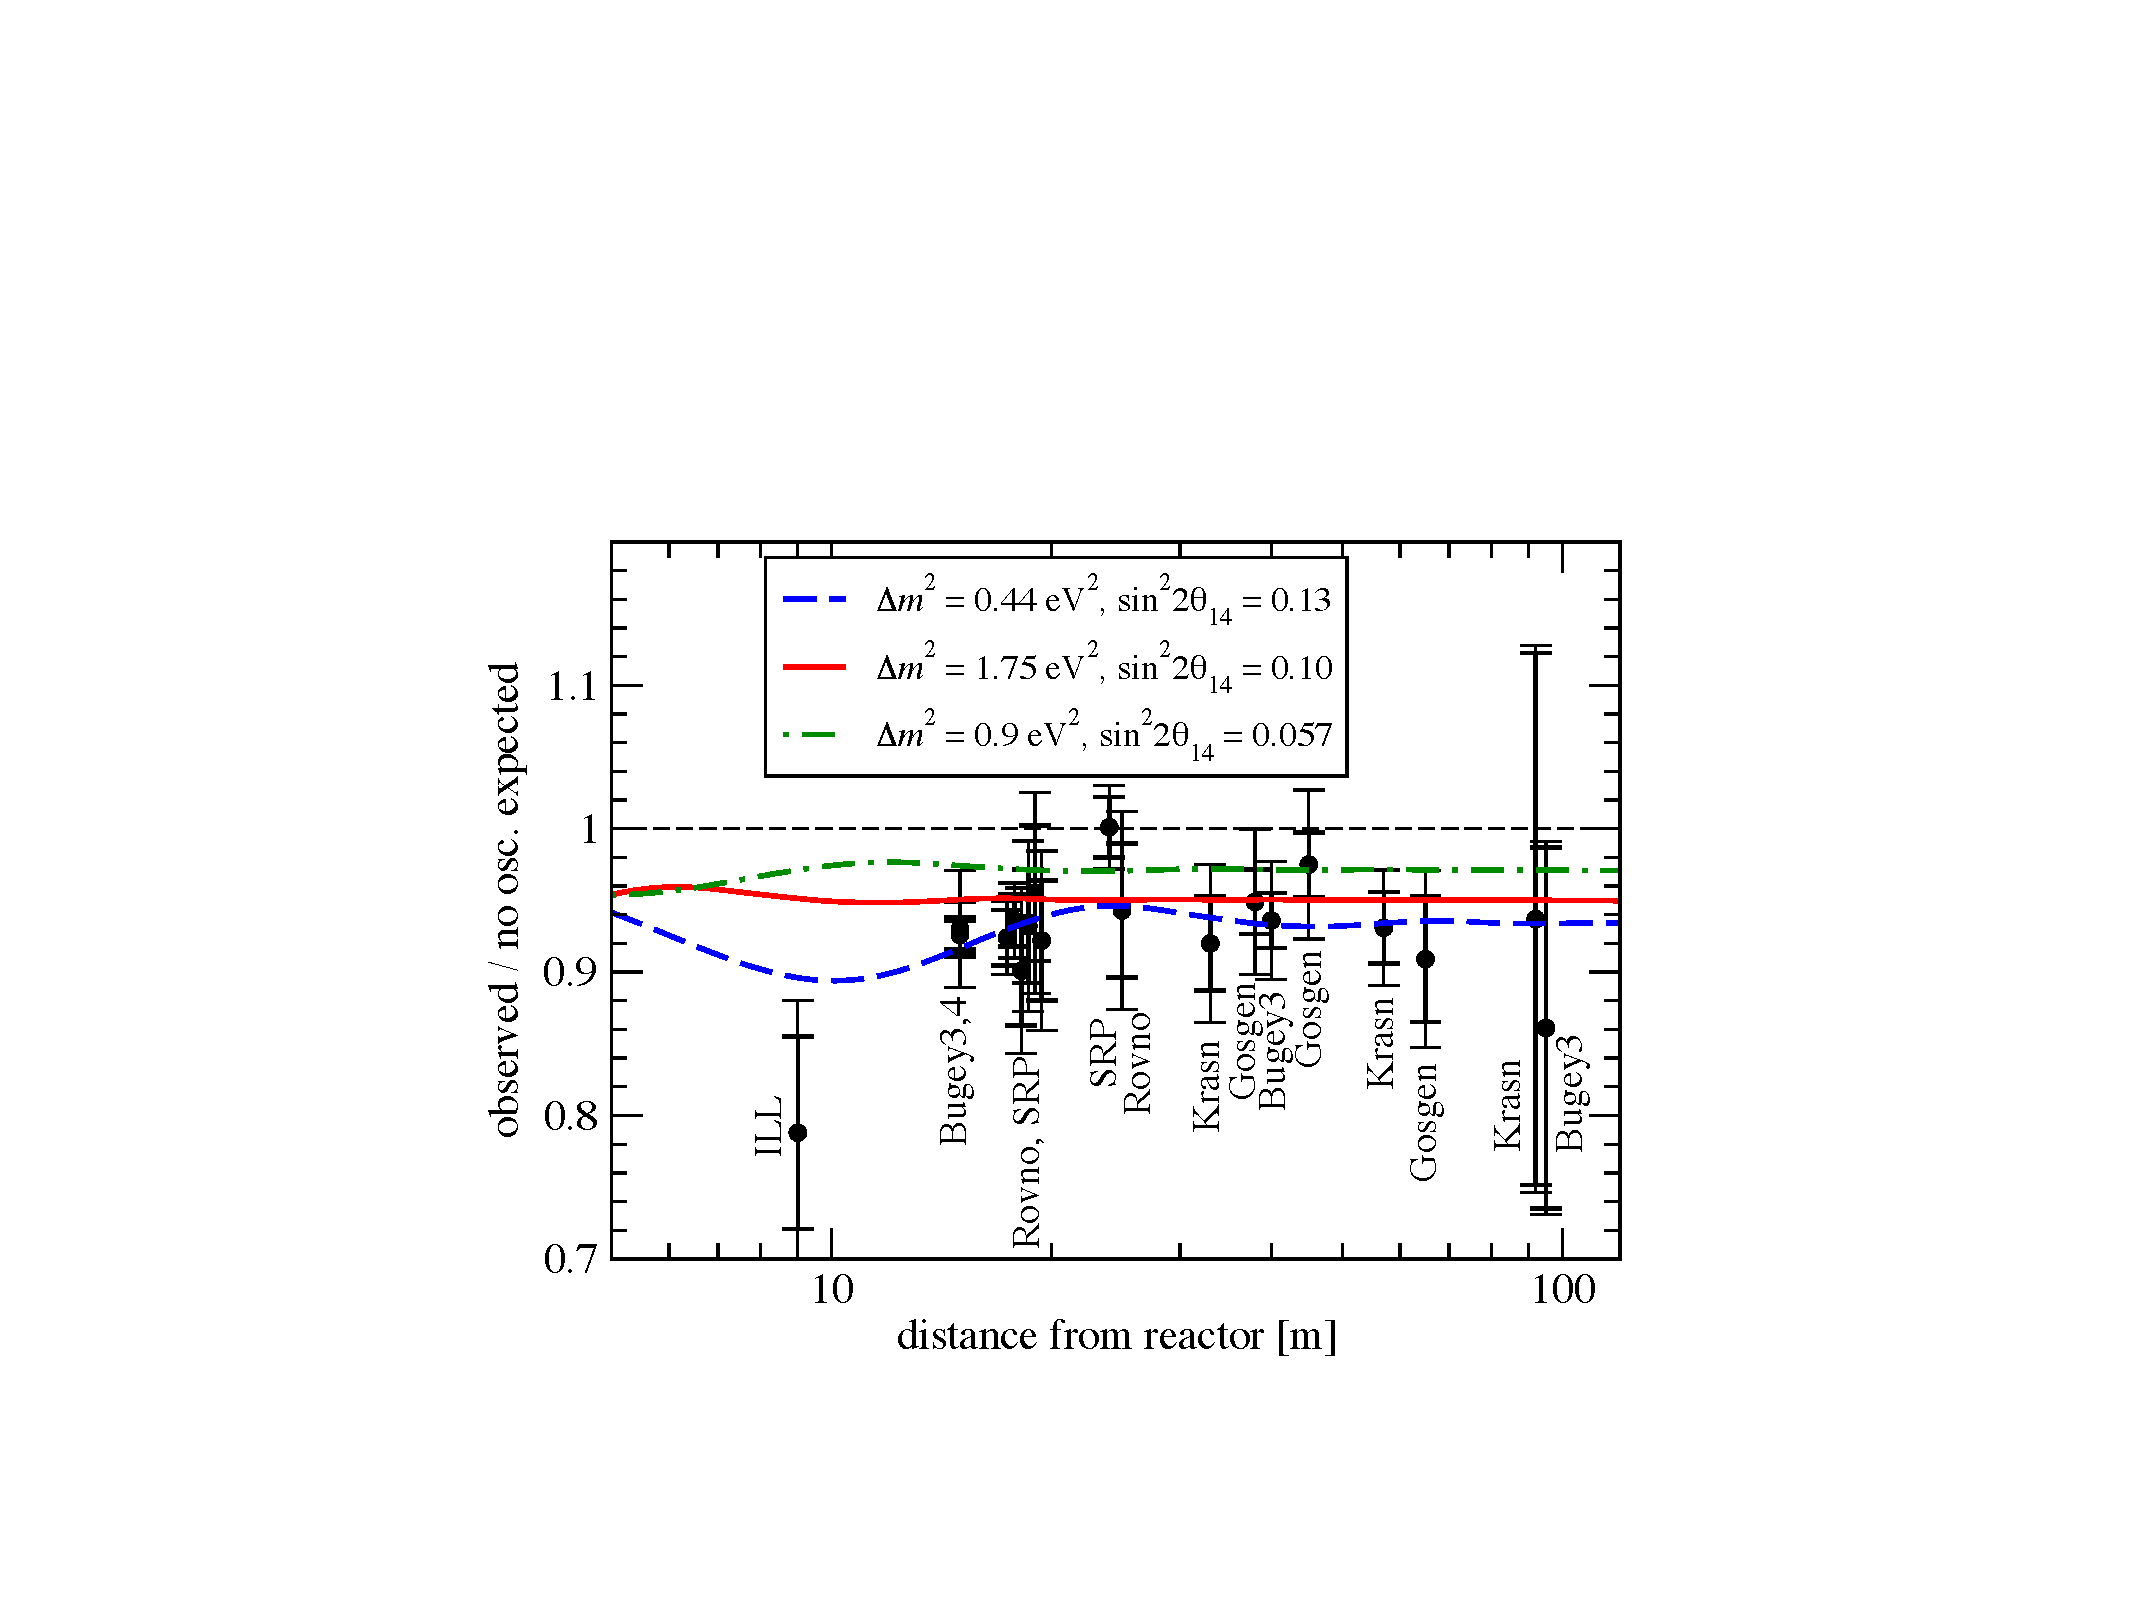
\includegraphics[width=0.75\linewidth]{figures/reactor.pdf}
      \caption{Fraction between observed and predicted $\bar{\nu}_{e}$ flux at several reactor neutrino experiments. Several models for sterile neutrino oscillation for different mass splitting terms and mixing angles are also shown.}
    \label{fig:reactor}
    \end{figure}
    
    This anomaly was first confirmed by a blind analysis of the Daya Bay collaboration \cite{An:2015nua} and then observed also by the RENO and Double Chooz detectors. More recently, these three experiments have also observed an excess of events (\emph{bump}) around 5~MeV. 
    In order to clarify the nature of the flux deficit, the Daya Bay experiment was able to correlate the antineutrino flux with the fuel composition in the reactor. The fuel evolves with time: the main fissile component, $^{235}$U, gets smaller, while the $^{239}$Pu increases. The model used to predict the inverse beta-decay yield is 3.1$\sigma$ in disagreement with data \cite{An:2017osx}. If the deficit is caused by sterile neutrinos, then it should not depend on the fissile material and the sterile neutrino hypothesis cannot be used to explain the fuel evolution model discrepancy. A combined analysis of Daya Bay and NEOS data hints to excess production of $^{235}$U as an explanation for the 5~MeV bump \cite{Huber:2016xis}. 
    
    \begin{figure}[htbp]
      \centering
      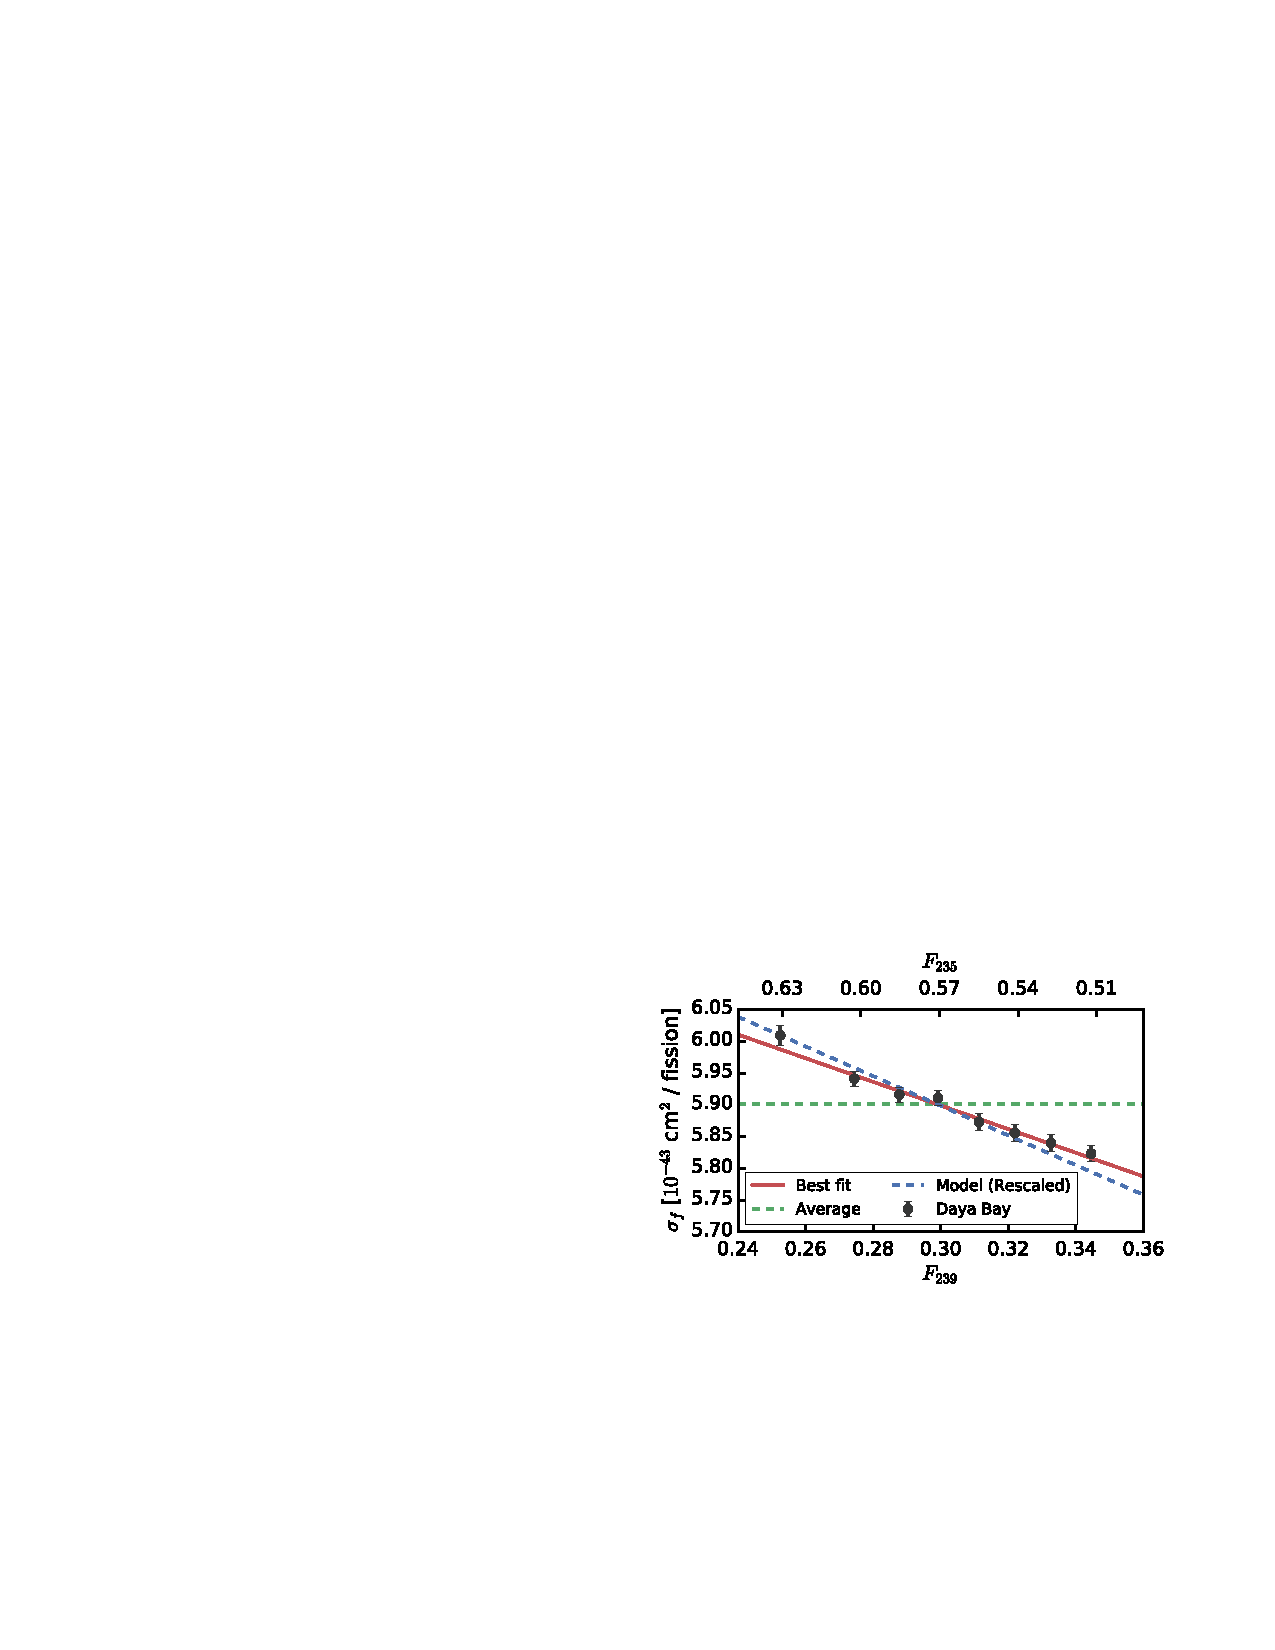
\includegraphics[width=0.75\linewidth]{figures/dayabay.pdf}
      \caption{Inverse $\beta$-decay yield per fission, $\sigma_f$, versus effective $^{239}$Pu (lower axis) or $^{235}$U (upper axis) fission fraction. From \cite{An:2017osx}.}
    \label{fig:dayabay}
    \end{figure}
    
    A new generation of reactor neutrino experiments should definitely solve the reactor anomaly. In particular, experiments like PROSPECT \cite{Ashenfelter:2015uxt} and SoLi$\partial$ \cite{Abreu:2017bpe}, will be placed very close to small fission cores and they will be sensitive to eventual short-baseline sterile neutrino oscillations.

\section{Constraints on the (3+1) model}

In the presence of a sterile neutrino, its mixing with the active flavours would affect the $\nu_e$ appearance, the $\nu_e$ disappearance, and the $\nu_{\mu}$ disappearance probabilities. However, the combined analysis of MINOS, Daya Bay, and Bugey-3 $\nu_{\mu}$ disappearance data \cite{Adamson:2016jku} also excludes the best-fit point. A recent result from IceCube \cite{TheIceCube:2016oqi} further restricts the available parameter space, leaving little room for the $(3+1)$ hypothesis. 
The tension emerges both by comparing appearance and disappearance experiment (Figure \ref{fig:disapp}) and by comparing $\nu_e$ data ($\nu_e\rightarrow\nu_e$, $\nu_e\rightarrow\nu_{\mu}$) and $\nu_{\mu}$ data ($\nu_{\mu}\rightarrow\nu_{\mu}$) (Figure \ref{fig:nue_vs_numu}). A global analysis \cite{Dentler:2018sju} excludes the $(3+1)$ model at $4.7\sigma$ level.

\begin{figure}[htbp]
  \begin{subfigure}{0.48\textwidth}
    \begin{center}
    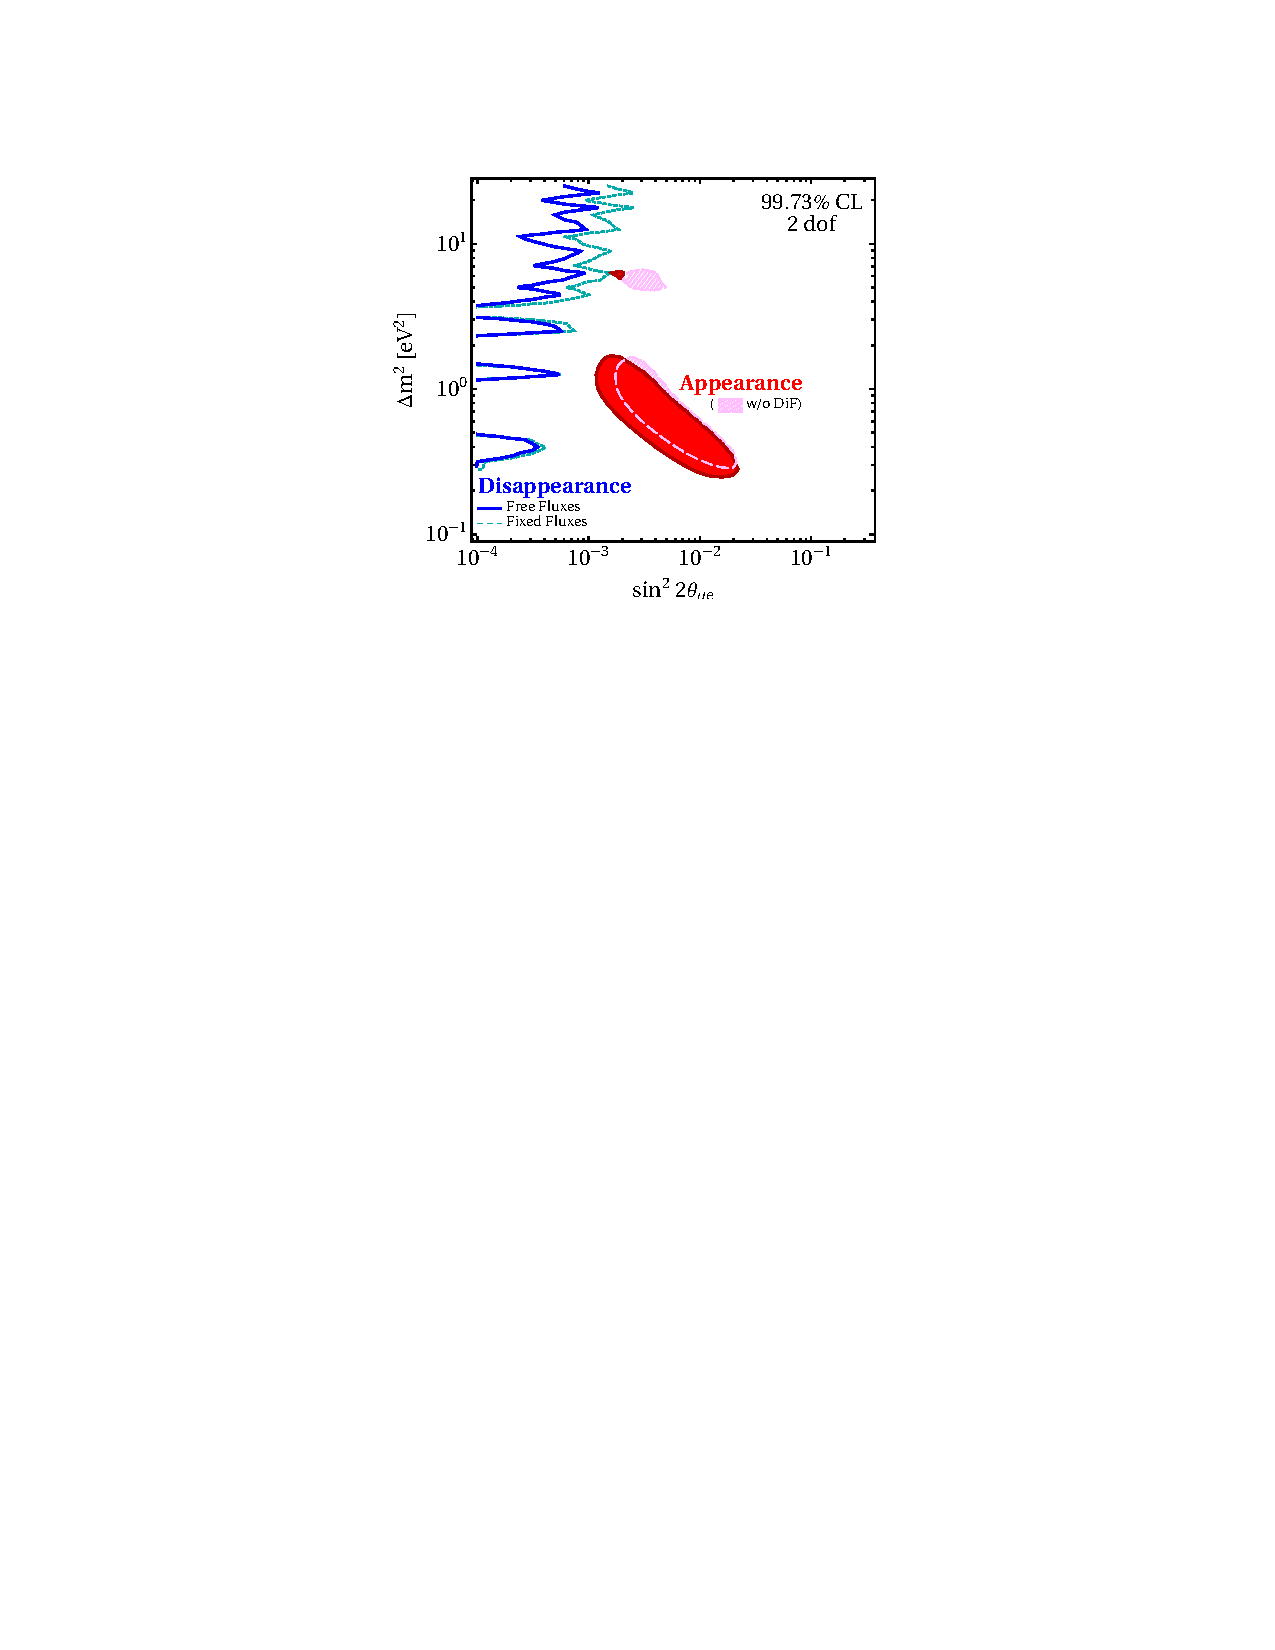
\includegraphics[width=\linewidth]{figures/disapp.pdf}
    \caption{Comparison between regions allowed by appearance results (filled red region) and regions excluded by disappearance results (solid blue line).}\label{fig:disapp}
    \end{center}
  \end{subfigure}\hfill
  \begin{subfigure}{0.48\textwidth}
    \begin{center}
    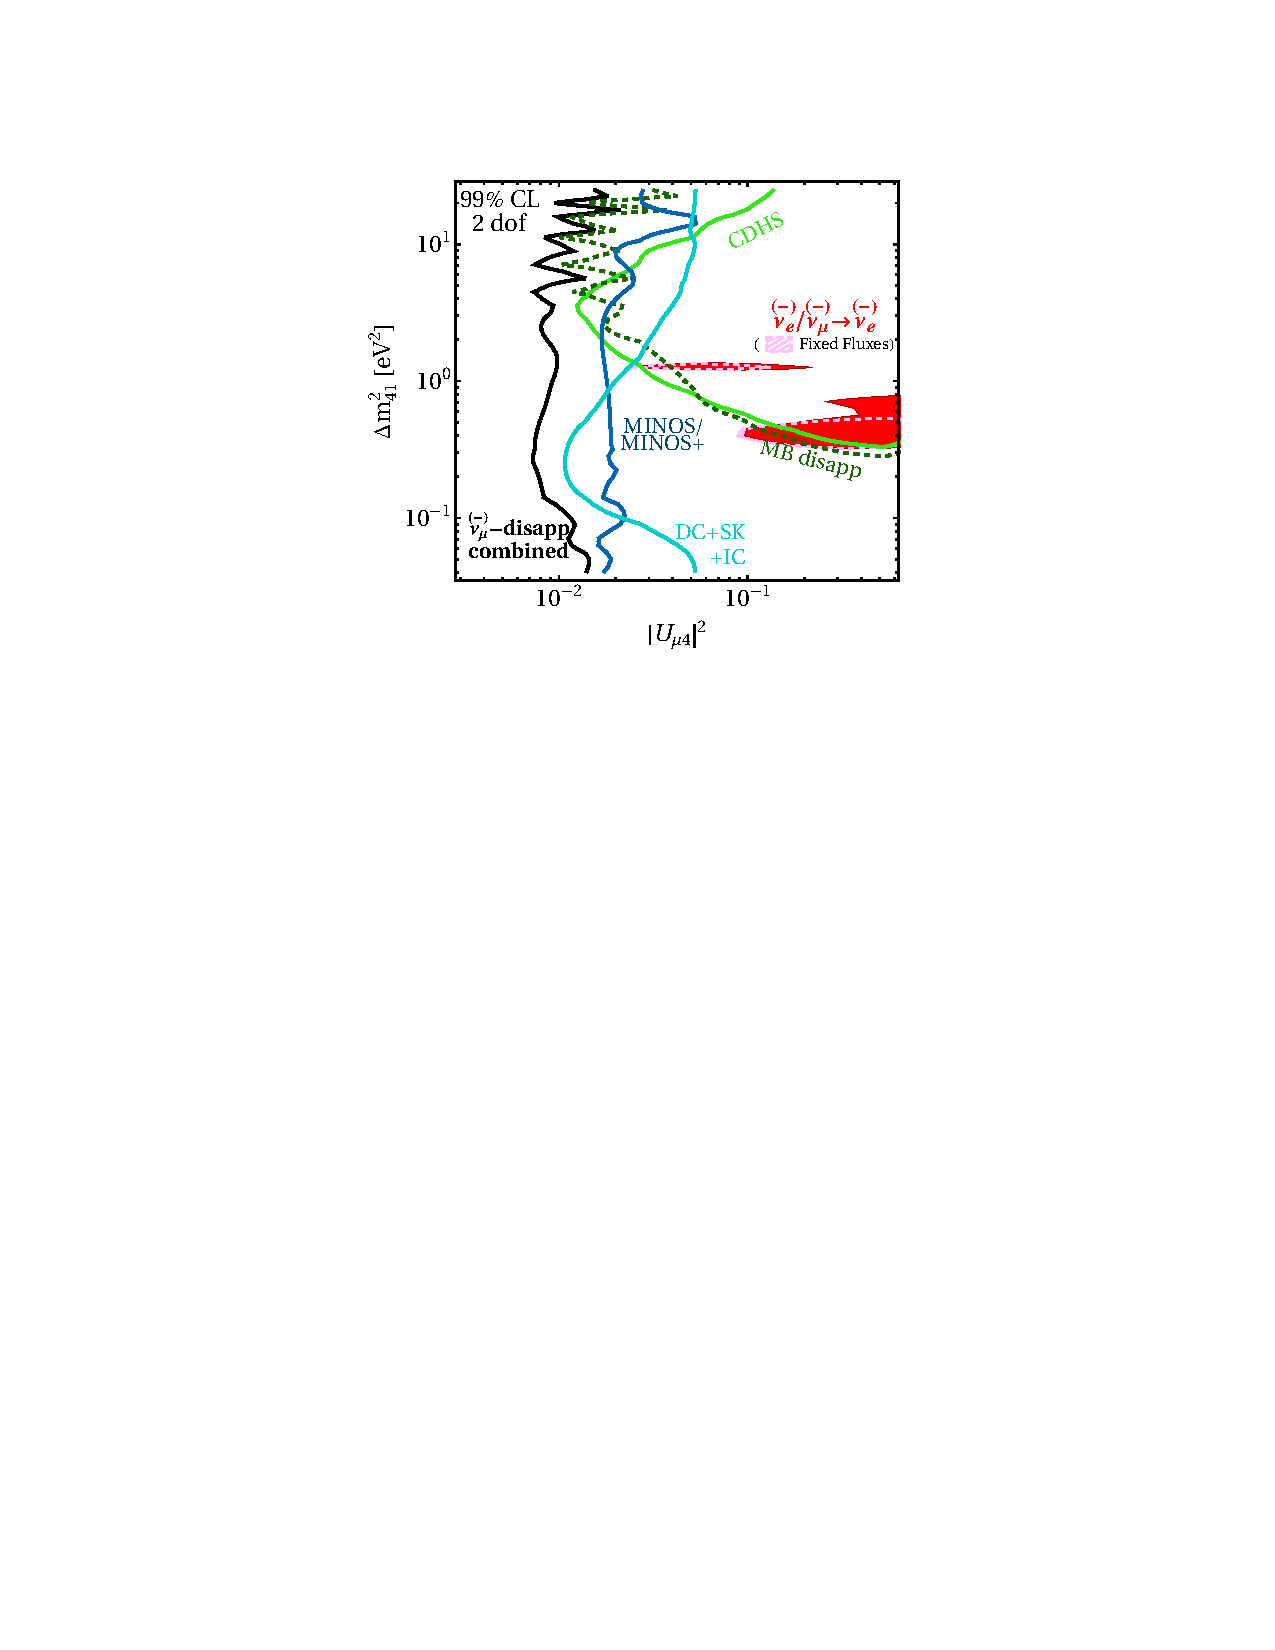
\includegraphics[width=\linewidth]{figures/nuenumu.pdf}
    \caption{Comparison between regions allowed by $\nu_e$ data ($\nu_e\rightarrow\nu_e$ and $\nu_e\rightarrow\nu_{\mu}$, filled red region) and regions excluded by $\nu_{\mu}$ disappearance data (solid lines).}\label{fig:nue_vs_numu}
    \end{center}
  \end{subfigure}
  \caption{There is a severe tension between appearance and disappearance results within the $(3+1)$ model. The free (fixed) fluxes lines of the plots on the left refer to the constraining (or not) of the reactor fluxes in the fits. Adapted from \cite{Dentler:2018sju}.}
\end{figure}

Other explanations have then been proposed for the excess: $3+N$ sterile neutrinos with $N>1$ \cite{Conrad:2012qt}, CPT violation \cite{Kostelecky:2011gq}, and resonant neutrino oscillations \cite{Asaadi:2017bhx} among the others. The explanation of the excess with the presence of a new particle decaying or scattering in the detector is severely constrained by kinematic arguments \cite{Jordan:2018qiy}.

\vspace{1em}

In summary, after the definitive confirmation of neutrino oscillations, achieved by employing different detection techniques, a series of new experiments collected data not fully compatible with a three-flavour scenario. In particular, a combined analysis of the LSND and MiniBooNE data gives a $6.0\sigma$ significance for an excess of electron-like events. This result is however in tension with other experiments if interpreted as the oscillation into a sterile neutrino state. 

Other experiments have also performed measurements not fully in agreement with the theoretical expectations, using both reactor antineutrinos and neutrinos from radioactive isotopes, but a coherent explanation for these anomalies still has to be provided. 